\documentclass{article}
\usepackage{booktabs}
\usepackage{multirow}
\usepackage{multicol}
\usepackage[table]{xcolor}
\usepackage{colortbl}
\usepackage[backend=biber,natbib=true,style=alphabetic,maxbibnames=50]{biblatex}
\addbibresource{/home/nqbh/reference/bib.bib}
\usepackage[utf8]{vietnam}
\usepackage{tocloft}
\usepackage{tcolorbox}

\setlength{\parindent}{0pt}


\usepackage{tikz}
\usetikzlibrary{arrows.meta}

\usepackage{minted}

\usepackage{listings}
\usepackage{xcolor}

\lstset{
    language=C++,                    % Ngôn ngữ lập trình
    basicstyle=\ttfamily\footnotesize, % Cỡ chữ nhỏ hơn
    keywordstyle=\color{blue},        % Màu từ khóa
    commentstyle=\color{gray},        % Màu chú thích
    stringstyle=\color{red},          % Màu chuỗi ký tự
    numbers=left,                     % Hiển thị số dòng bên trái
    numberstyle=\tiny\color{gray},    % Định dạng số dòng
    stepnumber=1,                     % Mỗi dòng đều có số dòng
    breaklines=true,                   % Tự động xuống dòng nếu quá dài
    frame=single                      % Đóng khung mã nguồn
}

\renewcommand{\cftsecleader}{\cftdotfill{\cftdotsep}}
\usepackage[colorlinks=true,linkcolor=blue,urlcolor=red,citecolor=magenta]{hyperref}
\usepackage{amsmath,amssymb,amsthm,enumitem,float,graphicx,mathtools,tikz}
\usetikzlibrary{angles,calc,intersections,matrix,patterns,quotes,shadings}
\allowdisplaybreaks
\newtheorem{assumption}{Assumption}
\newtheorem{baitoan}{}
\newtheorem{cauhoi}{Câu hỏi}
\newtheorem{conjecture}{Conjecture}
\newtheorem{corollary}{Corollary}
\newtheorem{dangtoan}{Dạng toán}
\newtheorem{definition}{Definition}
\newtheorem{dinhly}{Định lý}
\newtheorem{dinhnghia}{Định nghĩa}
\newtheorem{example}{Example}
\newtheorem{ghichu}{Ghi chú}
\newtheorem{hequa}{Hệ quả}
\newtheorem{giathuyet}{Giả thuyết}
\newtheorem{chungminh}{Chứng minh}
\newtheorem{hypothesis}{Hypothesis}
\newtheorem{lemma}{Lemma}
\newtheorem{luuy}{Lưu ý}
\newtheorem{nhanxet}{Nhận xét}
\newtheorem{baitap}{Bài tập}
\newtheorem{notation}{Notation}
\newtheorem{note}{Note}
\newtheorem{principle}{Principle}
\newtheorem{problem}{Problem}
\newtheorem{proposition}{Proposition}
\newtheorem{question}{Question}
\newtheorem{remark}{Remark}
\newtheorem{theorem}{Theorem}
\newtheorem{vidu}{Ví dụ}
\usepackage[left=1cm,right=1cm,top=5mm,bottom=5mm,footskip=4mm]{geometry}
\def\labelitemii{$\circ$}
\DeclareRobustCommand{\divby}{%
	\mathrel{\vbox{\baselineskip.65ex\lineskiplimit0pt\hbox{.}\hbox{.}\hbox{.}}}%
}
\setlist[itemize]{leftmargin=*}
\setlist[enumerate]{leftmargin=*}

\title{CHUYÊN ĐỀ: LÝ THUYẾT ĐỒ THỊ} 
\author{Đặng Phúc An Khang\footnote{ Email: {\tt ankhangluonvuituoi@gmail.com}. Tây Ninh, Việt Nam.}}
\date{\today}

\begin{document}
\maketitle
\begin{abstract}
	
	
	\textbf{Code:}
	\begin{quote}
		\begin{itemize}
			\item C{\tt/}C++: \url{https://github.com/GrootTheDeveloper/OLP-ICPC/tree/master/2025/C%2B%2B}.
			\item Python: \url{}\\
		\end{itemize}
	\end{quote}
	
	\textbf{Tài khoản trên các Online Judge:}
	\begin{quote}
    	\begin{itemize}
			\item Codeforces: \url{https://codeforces.com/profile/vuivethoima}.
			\item VNOI: \url{oj.vnoi.info/user/Groot}.
			\item IUHCoder: \url{oj.iuhcoder.com/user/ankhang2111}.
			\item MarisaOJ: \url{https://marisaoj.com/user/grootsiuvip/submissions}.
			\item CSES: \url{https://cses.fi/user/212174}.
			\item UMTOJ: \url{sot.umtoj.edu.vn/user/grootsiuvip}.
			\item SPOJ: \url{www.spoj.com/users/grootsiuvip/}.
			\item POJ: \url{http://poj.org/userstatus?user_id=vuivethoima}.
			\item ATCoder: \url{https://atcoder.jp/users/grootsiuvip}
			\item OnlineJudge.org: \url{vuivethoima}
			\item updating...
		\end{itemize}
	\end{quote}
    
\end{abstract}
\tableofcontents

%------------------------------------------------------------------------------%

\section{Preliminaries -- Kiến thức chuẩn bị}

\textbf{\textsf{Resources -- Tài nguyên.}}
\begin{enumerate}
	\item \cite{CP10}. \textit{CP10. Competitive Programming} \url{https://drive.google.com/drive/folders/1MTEVHT-7nBnMJ7C9LgyAR_pEVSE3FlKz?fbclid=IwAR3TovIj2rKCRe1a4oZxW-LQCoEoVkipVAvCzwrr0nJ6GzcAd47P6LO1Rwc}
	
	\item \cite{cp-algorithms}. \textit{Algorithms for Competitive Programming} \url{https://cp-algorithms.com}

    \item \cite{VNOI-WIKI}. \textit{Thư viện VNOI} \url{https://wiki.vnoi.info}



\end{enumerate}


%------------------------------------------------------------------------------%
\section{Kiến thức}
\subsection{Giới thiệu về đồ thị và thuật toán DFS}

\subsubsection{Lý thuyết đồ thị là gì?}

\begin{dinhnghia}
    Lý thuyết đồ thị là một nhánh của toán học, cụ thể thuộc toán rời rạc. Lý thuyết đồ thị chuyên nghiên cứu các bài toán liên quan đến việc biểu diễn và phân tích các sự vật, hiện tượng hoặc trạng thái có mối quan hệ lẫn nhau thông qua mô hình đồ thị.
\end{dinhnghia}
\begin{vidu}
    Mạng lưới giao thông, cây phả hệ (cây gia phả), mạng máy tính, sơ đồ tổ chức, v.v.
\end{vidu}

\subsubsection{Một số khái niệm căn bản trong lý thuyết đồ thị}

\begin{enumerate}
    \item \textbf{Đỉnh:} Được biểu diễn nhằm mục đích thể hiện sự vật, sự việc hay một trạng thái.
    \item \textbf{Cạnh:} Biểu diễn cho mối quan hệ giữa 2 đỉnh với nhau. \textbf{Lưu ý:} Giữa 2 đỉnh trong đồ thị có thể có cạnh, không có, hoặc có thể có nhiều cạnh với nhau. Cạnh được chia thành 2 dạng:
    \begin{enumerate}
        \item \textbf{Cạnh vô hướng:} Nếu một cạnh vô hướng nối 2 đỉnh $u$ và $v$, thì $u$ có thể đến $v$ trực tiếp vầ ngược lại.
        \item \textbf{Cạnh có hướng:} Nếu một cạnh có hướng nối từ đỉnh $u$ đến đỉnh $v$, thì ta có thể đi trực tiếp từ $u$ đến $v$, nhưng không thể đi ngược lại từ $v$ đến $u$ trừ khi có một cạnh khác từ $v$ đến $u$.
    \end{enumerate}
    \item \textbf{Đường đi:} Một đường đi là một danh sách các đỉnh $x_1, x_2, x_3, x_4,\dots, x_k$. Trong đó 2 đỉnh $x_i$ và $x_{i + 1}$ thì có một đường nối trực tiếp để đi từ $x_i$ $\rightarrow$ $x_{i + 1}$.
    \item \textbf{Trọng số:} Là một giá trị trên cạnh (hoặc trên đỉnh) nhằm thể hiện một thông số nào đó với bài toán ta đang xét.
\end{enumerate}

\subsubsection{Danh sách kề}

Một trong những cách phổ biến để biểu diễn đồ thị là sử dụng \textbf{danh sách kề (adjacency list)}. Cách biểu diễn này đặc biệt hiệu quả đối với đồ thị thưa \href{https://en.m.wikipedia.org/wiki/Sparse_graph}{(sparse graph)}.


Cụ thể, ta sử dụng cấu trúc dữ liệu \texttt{vector<int> adj[u]} trong C++, trong đó:

\begin{itemize}
    \item Mỗi phần tử \texttt{adj[u]} là một vector chứa các đỉnh kề với đỉnh $u$.
    \item Nghĩa là nếu có cạnh nối từ đỉnh $u$ đến đỉnh $v$ thì $v$ sẽ xuất hiện trong \texttt{adj[u]}.
    \item Đối với đồ thị vô hướng, nếu có cạnh giữa $u$ và $v$ thì cả $v \in \texttt{adj}[u]$ và $u \in \texttt{adj}[v]$.
\end{itemize}

\textbf{Ví dụ:}

Giả sử đồ thị vô hướng có các cạnh: $(1,2)$, $(1,3)$, $(2,4)$ thì danh sách kề sẽ là:

\begin{align*}
\texttt{adj[1]} &= \{2, 3\} \\
\texttt{adj[2]} &= \{1, 4\} \\
\texttt{adj[3]} &= \{1\} \\
\texttt{adj[4]} &= \{2\}
\end{align*}

\begin{figure}[H]
    \centering
    \includegraphics[width=0.2\textwidth]{img/b1/adjlist.png}
    \caption{Minh họa danh sách kề của đồ thị vô hướng vừa mô tả}
    \label{fig:adjlist}
\end{figure}

Cách biểu diễn này có độ phức tạp về bộ nhớ là $\mathcal{O}(n + m)$, với $n$ là số đỉnh và $m$ là số cạnh.

\subsubsection{Chu trình (Cycle)}
\begin{dinhnghia}
    Một \textbf{chu trình} là một đường đi bắt đầu và kết thúc tại cùng một đỉnh, trong đó không có đỉnh nào khác (ngoại trừ đỉnh đầu/cuối) được lặp lại.
\end{dinhnghia}
    \begin{itemize}
        \item Trong đồ thị vô hướng: chu trình là dãy đỉnh $v_1 \rightarrow v_2 \rightarrow \dots \rightarrow v_k \rightarrow v_1$ với $k \geq 3$.
        \item Trong đồ thị có hướng: các cung phải có hướng phù hợp với trình tự chu trình.
    \end{itemize}
    
    Một chu trình được gọi là \textit{chu trình đơn giản} nếu không có cạnh hoặc đỉnh nào bị lặp lại (trừ đỉnh đầu/cuối).
    
\begin{figure}[H]
    \centering
    \includegraphics[width=0.4\textwidth]{img/b1/cycle.png}
    \caption{Minh họa chu trình của đồ thị vô hướng}
    \label{fig:cycle}
\end{figure}

\subsubsection{Thành phần liên thông \href{https://www.geeksforgeeks.org/dsa/strongly-connected-components/}{(Connected Component)}}
\begin{dinhnghia}

    Một \textbf{thành phần liên thông} là một tập con các đỉnh sao cho giữa mọi cặp đỉnh trong đó đều tồn tại một đường đi.
\end{dinhnghia}
    
\begin{itemize}
    \item Với đồ thị vô hướng: liên thông nếu có đường đi giữa mọi cặp đỉnh.
    \item Với đồ thị có hướng:
        \begin{itemize}
            \item \textit{Liên thông mạnh} nếu tồn tại đường đi theo chiều từ mọi đỉnh đến mọi đỉnh khác.
            \item \textit{Liên thông yếu} nếu bỏ hướng trên các cạnh thì đồ thị trở nên liên thông.
        \end{itemize}
\end{itemize}

\begin{figure}[H]
    \centering
    \includegraphics[width=0.4\textwidth]{img/b1/SCC.png}
    \caption{Minh họa thành phần liên thông mạnh của đồ thị có hướng}
    \label{SCC}
\end{figure}

\subsubsection{Bậc của đỉnh (Degree)}
\begin{itemize}
    \item Trong đồ thị vô hướng, bậc của một đỉnh là số cạnh nối với nó.
    \item Trong đồ thị có hướng:
        \begin{itemize}
            \item \textit{Bậc vào} (in-degree): số cung đi vào đỉnh.
            \item \textit{Bậc ra} (out-degree): số cung đi ra từ đỉnh.
        \end{itemize}
\end{itemize}

\subsubsection{Đường đi đơn giản (Simple Path)}
Một \textbf{đường đi đơn giản} là đường đi không đi qua một đỉnh nào hai lần (trừ khi là chu trình).

\subsubsection{Cây (Tree)}
\begin{dinhnghia}
    
    Một \textbf{cây} là một đồ thị vô hướng liên thông và không có chu trình.
    
\end{dinhnghia}
Tính chất quan trọng của cây:
\begin{itemize}
    \item Với $n$ đỉnh, cây có đúng $n - 1$ cạnh.
    \item Có duy nhất một đường đi giữa hai đỉnh bất kỳ.
\end{itemize}

\begin{figure}[H]
    \centering
    \includegraphics[width=0.4\textwidth]{img/b1/treegraph.png}
    \caption{Phân biệt Cây và Đồ thị (không phải cây)}
    \label{treegraph}
\end{figure}

\subsubsection{Đồ thị vô chu trình (Acyclic Graph).}
Đồ thị gọi là \textbf{vô chu trình} nếu không tồn tại chu trình nào trong nó.
\begin{itemize}
    \item Với đồ thị \textbf{vô hướng}, một đồ thị được xem là \textbf{Acyclic Graph} nếu không tồn tại dãy các đỉnh $v_1 \rightarrow v_2 \rightarrow \dots \rightarrow v_k \rightarrow v_1$ với $k \geq 3$ và các cạnh liên tiếp nối các đỉnh đó.
    \item Một đồ thị vô hướng đơn giản gồm hai đỉnh được nối với nhau bằng một cạnh cũng là một \textbf{Acyclic Graph}, vì không tồn tại chu trình nào (phải có ít nhất 3 đỉnh để hình thành chu trình trong đồ thị vô hướng).
    \item Đồ thị có hướng vô chu trình gọi là \textbf{DAG} (Directed Acyclic Graph). Nghĩa là một đồ thị có hướng không chứa bất kỳ chu trình nào tuân theo chiều các cung.
    \item Cây là một DAG, nhưng không phải tất cả DAG đều là cây.
\end{itemize}

\begin{figure}[H]
    \centering
    \includegraphics[width=0.6\textwidth]{img/b1/treevsdag.jpg}
    \caption{Phân biệt Cây và DAG}
\end{figure}

\subsubsection{Đồ thị đơn (Simple Graph).}
Đồ thị đơn là đồ thị không có \emph{cạnh lặp} giữa cùng một cặp đỉnh và không có \emph{khuyên} (loop – cạnh nối đỉnh với chính nó).

\subsubsection{Đa đồ thị (Multigraph).}
Đa đồ thị cho phép tồn tại \emph{nhiều cạnh song song} giữa hai đỉnh và/hoặc khuyên.  
Thường dùng để mô hình hoá các mạng có nhiều kênh kết nối.

\begin{figure}[H]
    \centering
    \includegraphics[width=0.2\textwidth]{img/b1/multigraph.png}
    \caption{Minh họa Đa đồ thị}
    \label{multigraph}
\end{figure}

\subsubsection{Đồ thị đầy đủ (Complete Graph).}
Đồ thị vô hướng \(K_n\) có \(n\) đỉnh, trong đó mọi cặp đỉnh phân biệt đều được nối bởi một cạnh. 

Số cạnh là \(\dfrac{n(n-1)}{2}\).  

Đồ thị có hướng đầy đủ có \(n(n-1)\) cung.

\begin{figure}[H]
    \centering
    \includegraphics[width=0.2\textwidth]{img/b1/CG.png}
    \caption{Minh họa đồ thị đầy đủ}
    \label{CG}
\end{figure}

\subsubsection{Đồ thị hai phía (Bipartite Graph).}
Một \textbf{đồ thị hai phía} là đồ thị mà tập đỉnh có thể chia thành hai tập rời $U$ và $V$ sao cho mọi cạnh đều nối một đỉnh từ $U$ đến một đỉnh từ $V$.

\begin{figure}[H]
    \centering
    \includegraphics[width=0.5\textwidth]{img/b1/biparitegraph.png}
    \caption{Phân biệt đồ thị hai phía}
    \label{biparite}
\end{figure}

\subsubsection{Đồ thị hai phía đầy đủ (Complete Bipartite Graph).}
Cho hai tập đỉnh rời \(U\) và \(V\) với \(|U| = m,\;|V| = n\).  
Đồ thị \(K_{m,n}\) chứa mọi cạnh nối một đỉnh của \(U\) với một đỉnh của \(V\) và \emph{không có cạnh nội bộ} trong \(U\) hay \(V\).  
Tổng số cạnh: \(m\,n\).

\begin{figure}[H]
    \centering
    \includegraphics[width=0.4\textwidth]{img/b1/completebiparitegraph.png}
    \caption{Minh họa đồ thị hai phía đầy đủ}
    \label{CBG}
\end{figure}

\subsubsection{Đồ thị vòng (Cycle Graph)}
Đồ thị vòng ký hiệu \(C_n\;(n \ge 3)\) là đồ thị vô hướng gồm \(n\) đỉnh
\(\{v_1,v_2,\dots ,v_n\}\) và \(n\) cạnh
\[
E = \bigl\{\{v_1,v_2\},\{v_2,v_3\},\dots ,\{v_{n-1},v_n\},\{v_n,v_1\}\bigr\}.
\]

\begin{itemize}
    \item Mỗi đỉnh có bậc \(2\) – \(C_n\) là đồ thị \(2\)-chính quy.
    \item \(C_n\) chứa đúng một chu trình đơn giản độ dài \(n\).
    \item \(C_n\) là \textbf{bipartite} khi và chỉ khi \(n\) chẵn.
    \item Số cạnh \(m = n\); số đỉnh \(n\); đường kính (diameter)  
          \(\operatorname{diam}(C_n) = \bigl\lfloor n/2 \bigr\rfloor\).
    \item Tồn tại cây khung nhỏ nhất với trọng số tổng bằng \(n-1\) nếu mọi cạnh có trọng số \(1\).
\end{itemize}

\begin{figure}[H]
    \centering
    \includegraphics[width=0.4\textwidth]{img/b1/CGvsAG.png}
    \caption{Minh họa CG và AG}

\end{figure}
\subsubsection{Rừng (Forest).}
Một \textbf{rừng} là đồ thị vô hướng \emph{không chứa chu trình} nhưng \emph{không nhất thiết liên thông}.  
Mỗi thành phần liên thông của rừng là một \textbf{cây}.  
Nếu rừng có \(c\) cây và \(n\) đỉnh, nó có đúng \(n-c\) cạnh.


\begin{figure}[H]
    \centering
    \includegraphics[width=0.4\textwidth]{img/b1/treevsforest.jpg}
    \caption{Tree vs Forest}    
\end{figure}


\subsection{Thuật toán DFS}

Thuật toán DFS (Depth-First Search – Duyệt theo chiều sâu) là một trong những thuật toán cơ bản để duyệt hoặc tìm kiếm trên đồ thị. Ý tưởng chính là xuất phát từ một đỉnh ban đầu, đi sâu theo từng nhánh con của đồ thị cho đến khi không còn đỉnh nào có thể đi tiếp, sau đó quay lui để khám phá các nhánh khác.

DFS có thể được cài đặt đệ quy hoặc sử dụng ngăn xếp. Nó thường được dùng để:

\begin{itemize}
    \item Kiểm tra tính liên thông của đồ thị
    \item Tìm thành phần liên thông
    \item Phát hiện chu trình
    \item Tìm đường đi trong mê cung hoặc đồ thị
\end{itemize}

\subsubsection{Ý tưởng cài đặt thuật toán DFS}

DFS thường được cài đặt bằng đệ quy hoặc sử dụng ngăn xếp. Trong cài đặt đệ quy, ta cần một mảng đánh dấu để theo dõi các đỉnh đã được thăm nhằm tránh lặp vô hạn trong trường hợp đồ thị có chu trình.

\textbf{Các bước cơ bản trong cài đặt DFS đệ quy:}

\begin{enumerate}
    \item Khởi tạo một mảng \texttt{visited[]} để đánh dấu các đỉnh đã được duyệt, với ý nghĩa: \texttt{visited[u] = true / false} nếu đỉnh $u$ đã thăm / chưa thăm.
    \item Gọi hàm \texttt{DFS(u)} tại đỉnh bắt đầu $u$.
    \item Trong mỗi lần gọi:
    \begin{itemize}
        \item Đánh dấu \texttt{visited[u] = true}.
        \item Duyệt qua tất cả các đỉnh kề $v$ của $u$:
        \begin{itemize}
            \item Nếu $v$ chưa được thăm (\texttt{visited[v] == false}), đệ quy gọi \texttt{DFS(v)}.
        \end{itemize}
    \end{itemize}
\end{enumerate}

\subsubsection{Cài đặt DFS sử dụng đệ quy trong C++}

\begin{lstlisting}[language=C++, caption={Thuật toán DFS sử dụng đệ quy}, label={code:dfs}]
#include <iostream>
#include <vector>
using namespace std;

const int MAXN = 100005; // So dinh toi da
vector<int> adj[MAXN];   // Danh sach ke
bool visited[MAXN];      // Mang danh dau

void DFS(int u) {
    visited[u] = true;
    cout << "Tham dinh: " << u << endl;
    for (int v : adj[u]) {
        if (!visited[v]) {
            DFS(v);
        }
    }
}
int main() {
    int n, m; // so dinh va so canh
    cin >> n >> m;
    for (int i = 0; i < m; i++) {
        int u, v;
        cin >> u >> v;
        adj[u].push_back(v);
        adj[v].push_back(u); // Neu la do thi vo huong
    }
    for (int i = 1; i <= n; i++) {
        visited[i] = false;
    }
    // Goi DFS tu dinh 1 (hoac 1 dinh bat ky)
    DFS(1);

    return 0;
}
\end{lstlisting}

\textbf{Độ phức tạp: } $\mathcal{O}(V + E)$ với $V$ là số đỉnh, $E$ là số cạnh.

\subsubsection{Bài tập}
\begin{baitap}    
    \href{https://www.spoj.com/problems/MAKEMAZE/}{MAKEMAZE}
\end{baitap} 

\textbf{Đề bài}

Một mê cung hợp lệ là một mê cung có chính xác 1 lối vào và 1 lối ra  và phải tồn tại ít nhất một đường đi thỏa mãn từ lối vào đến lối ra. Cho một mê cung, hãy chỉ ra rằng mê cung có hợp lệ hay không. Nếu có, in ``valid'', ngược lại in ``invalid''

\textbf{Input}

Dòng đầu chứa một số nguyên $t$ $(1 \leq t \leq 10^4)$ là số lượng test cases. Sau đó với mỗi test case, dòng đầu chứa 2 số nguyên $m$ $(1 \leq m \leq 20)$ và $n$ $(1 \leq n \leq 20)$, lần lượt là số lượng hàng và cột trong mê cung. Sau đó, là mê cung $M$ với kích thước $m$ x $n$. $M[i][j] = '\#'$ đại diện cho bức tường, $M[i][j] = '.'$ đại diện cho ô trống có thể đi vào được.

\textbf{Output}

Với mỗi test case, tìm xem mê cung tương ứng là ``invalid'' hay ``valid''

\textbf{Example}

\paragraph{Input}
\begin{lstlisting}
 1
 4 4 
 ####
 #...  
 #.## 
 #.## 
\end{lstlisting}

\paragraph{Output}
\begin{lstlisting}
valid
\end{lstlisting}

%$\rightarrow$ ``valid''

\textbf{Phân tích bài toán}

Vì mê cung chỉ có chính xác 1 lối vào và 1 lối ra. Trước hết ta cần kiểm tra biên ngoài của mê cung, nếu có chính xác 2 ô '.' thì có thể đó là một mê cung hợp lệ. Ngược lại (có ít hơn hoặc nhiều hơn 1 ô '.' ở biên) ta có thể khẳng định rằng đó không phải là một mê cung hợp lệ. \\

Khi ta đã có giả thuyết rằng mê cung là hợp lệ, ta cần 2 biến \textit{start} và \textit{target} lần lượt lưu lại tọa độ $(x, y)$ của 2 ô ngoài biên. Áp dụng thuật toán DFS tại ô $start$, sau khi DFS nếu \textit{visited[target.first][target.second] = true} thì khẳng định rằng mê chung hợp lệ. Ngược lại, mê cung khônxg hợp lệ.
\begin{lstlisting}[language=C++, caption={Cài đặt C++ bài MAKEMAZE}, label={code:makemaze}]
#include <bits/stdc++.h>
#define int long long
#define endl "\n"
using namespace std;

const int MAXN = 21;
bool visited[MAXN][MAXN];

int dx[4] = {1, -1, 0, 0};
int dy[4] = {0, 0, 1, -1};

void dfs(pair<int, int> start, const vector<vector<char>> &a, int m, int n) {
    auto [x, y] = start;
    visited[x][y] = true;
    for (int i = 0; i < 4; i++) {
        int new_x = dx[i] + x;
        int new_y = dy[i] + y;
        if (new_x >= 1 && new_x <= m && new_y >= 1 && new_y <= n &&
            !visited[new_x][new_y] && a[new_x][new_y] == '.') {
            dfs({new_x, new_y}, a, m, n);
        }
    }
}

signed main() {
    int t; cin >> t;
    while (t--) {
        int m, n; cin >> m >> n;
        vector<vector<char>> a(m + 1, vector<char>(n + 1));
        for (int i = 1; i <= m; i++) {
            for (int j = 1; j <= n; j++) {
                cin >> a[i][j];
                visited[i][j] = false;
            }
        }

        pair<int, int> start = {-1, -1}, target = {-1, -1};
        int cnt = 0;

        for (int i = 1; i <= m; i++) {
            for (int j = 1; j <= n; j++) {
                if ((i == 1 || i == m || j == 1 || j == n) && a[i][j] == '.') {
                    if (start == make_pair(-1LL, -1LL)) start = {i, j};
                    else target = {i, j};
                    cnt++;
                }
            }
        }

        if (cnt != 2) {
            cout << "invalid" << endl;
            continue;
        } else {
            dfs(start, a, m, n);
            if (!visited[target.first][target.second]) cout << "invalid";
            else cout << "valid";
            cout << endl;
        }
    }
    return 0;
}

\end{lstlisting}

\subsection{Sắp xếp tô-pô \href{https://wiki.vnoi.info/algo/graph-theory/topological-sort.md}{(Topological Sorting)}}

Nội dung bài chủ yếu tham khảo/copy từ [VNOI WIKI] : \url{https://wiki.vnoi.info/algo/graph-theory/topological-sort.md}

\subsubsection{Định nghĩa}

\begin{dinhnghia}
Cho một đồ thị có hướng \( G = (V, E) \), sắp xếp tô-pô (topological sorting) là một ánh xạ từ tập đỉnh \( V \) vào tập các số nguyên \( \{1, 2, \dots, |V|\} \), sao cho với mọi cung \( (u, v) \in E \), ta có:
\[
\operatorname{order}(u) < \operatorname{order}(v).
\]
\end{dinhnghia}

\begin{dinhnghia}
    Sắp xếp tô-pô là cách sắp xếp các đỉnh của một đồ thị có hướng sao cho nếu có một mũi tên từ đỉnh \( u \) đến đỉnh \( v \), thì \( u \) phải đứng trước \( v \) trong thứ tự đó.
\end{dinhnghia}

Nói cách khác, thứ tự tô-pô là một hoán vị của các đỉnh sao cho mọi cung đều đi từ đỉnh đứng trước đến đỉnh đứng sau trong thứ tự này. Hay nếu một công việc \( u \) cần hoàn thành trước công việc \( v \), thì \( u \) phải xuất hiện trước \( v \) trong danh sách kết quả.



\begin{figure}[H]
    \centering
    \includegraphics[width=0.6\textwidth]{img/b2/topological_sort_img1.png}
    \caption{Minh họa sắp xếp Tô-pô}
\end{figure}

\subsubsection{Cảm hứng và Động cơ ứng dụng}

Sắp xếp tô-pô là một công cụ quan trọng trong việc mô hình hóa và giải quyết các bài toán liên quan đến \textbf{phụ thuộc thứ tự} giữa các đối tượng. Về bản chất, nó cho phép ta xác định một trình tự thực hiện hợp lệ sao cho mọi điều kiện tiên quyết đều được thỏa mãn trước khi thực hiện bước tiếp theo.

Một ứng dụng thực tế điển hình là trong \textbf{lập kế hoạch công việc}. Khi một tập hợp các công việc có quan hệ phụ thuộc lẫn nhau, ta cần xác định thứ tự thực hiện sao cho mỗi công việc chỉ bắt đầu sau khi tất cả các công việc phụ thuộc của nó đã hoàn thành.

\textbf{Ví dụ minh họa:} Trong chương trình đào tạo đại học, sinh viên cần hoàn thành nhiều học phần để tốt nghiệp. Một số học phần là điều kiện tiên quyết cho các học phần khác. Chẳng hạn:
\begin{itemize}
    \item Để học được môn ``Giới thiệu về thuật toán'', sinh viên phải hoàn thành các môn: ``Nhập môn lập trình'', ``Cấu trúc dữ liệu'', ``Nhập môn thuật toán'', v.v.
\end{itemize}

Ta có thể xây dựng một đồ thị có hướng, trong đó:
\begin{itemize}
    \item Mỗi đỉnh tương ứng với một học phần;
    \item Có một cung từ đỉnh \( u \) đến đỉnh \( v \) nếu học phần \( u \) là điều kiện tiên quyết của học phần \( v \).
\end{itemize}

Khi đó, việc tìm một sắp xếp tô-pô của đồ thị này sẽ cho ta một thứ tự học hợp lệ. Nếu không tồn tại sắp xếp tô-pô (tức đồ thị có chu trình), điều đó phản ánh sự xung đột hoặc vòng lặp trong điều kiện tiên quyết giữa các môn học - một cấu trúc bất hợp lệ trong thiết kế chương trình đào tạo.

\begin{ghichu}
Sắp xếp tô-pô không xử lý các xung đột tài nguyên như trùng lịch học, mà chỉ đảm bảo mối quan hệ thứ tự phụ thuộc.
\end{ghichu}


\begin{ghichu}
Chỉ tồn tại sắp xếp tô-pô nếu và chỉ nếu đồ thị là DAG (Directed Acyclic Graph).

\end{ghichu}


\subsubsection{Chứng minh điều kiện tồn tại thứ tự Tô-pô}

\begin{giathuyet}
    Một đồ thị có hướng tồn tại thứ tự Tô-pô khi và chỉ khi nó là một \textbf{DAG}.
\end{giathuyet}

\begin{giathuyet}
    Đồng nghĩa, mọi DAG đều tồn tại ít nhất một thứ tự Tô-pô.
\end{giathuyet}

\begin{giathuyet}
    Có thể tìm được một thứ tự Tô-pô bằng thuật toán trong thời gian tuyến tính \( \mathcal{O}(V + E) \).
\end{giathuyet}

\begin{chungminh}
Ta sẽ chứng minh hai chiều của giả thuyết chính.

\textbf{Chiều thuận:} Nếu đồ thị \( G \) có chu trình, thì không thể tồn tại thứ tự tô-pô.

Giả sử tồn tại chu trình \( v_1 \to v_2 \to \dots \to v_n \to v_1 \). Khi đó, theo định nghĩa của thứ tự tô-pô, ta có:
\[
\operatorname{order}(v_1) < \operatorname{order}(v_2) < \dots < \operatorname{order}(v_n) < \operatorname{order}(v_1),
\]
tức là \( \operatorname{order}(v_1) < \operatorname{order}(v_1) \), mâu thuẫn. Vậy, nếu có chu trình, không tồn tại thứ tự tô-pô.\\

\textbf{Chiều nghịch:} Nếu \( G \) là một DAG, thì tồn tại ít nhất một thứ tự tô-pô.

\begin{enumerate}
    \item Vì \( G \) không có chu trình, nên tồn tại ít nhất một đỉnh không có cung đi vào (bậc vào bằng 0). Nếu mọi đỉnh đều có bậc vào \(\geq 1\), thì bắt đầu từ một đỉnh bất kỳ, ta luôn đi được sang đỉnh khác (vì có cung đi vào), và cuối cùng sẽ đi thành một chu trình, mâu thuẫn với giả thiết \( G \) là DAG.

    \item Gọi đỉnh đó là \( u \). Đặt \( u \) là đỉnh đầu tiên trong thứ tự tô-pô.

    \item Loại bỏ \( u \) khỏi đồ thị cùng tất cả các cung đi ra từ \( u \). Đồ thị còn lại vẫn là DAG (vì việc xóa đỉnh không thể tạo ra chu trình mới).

    \item Áp dụng lại quá trình trên với đồ thị còn lại: luôn tồn tại đỉnh có bậc vào bằng 0, đưa nó vào tiếp theo trong thứ tự.

    \item Lặp lại cho đến khi tất cả các đỉnh được đưa vào thứ tự.

    \item Cuối cùng, ta thu được một thứ tự thỏa mãn định nghĩa sắp xếp tô-pô.
\end{enumerate}

\begin{figure}[H]
    \centering
    \includegraphics[width=0.6\textwidth]{img/b2/topological_sort_img2.png}
    \caption{Minh họa chứng minh chiều nghịch}
\end{figure}
\textbf{Kết luận:} Với mỗi DAG, luôn tồn tại ít nhất một thứ tự tô-pô.
\end{chungminh}

\subsubsection{Bài tập}
\begin{baitap}
    TOPOSORT - Sắp xếp TOPO
\end{baitap}

\textbf{Đề bài}
Cho đồ thị có hướng không chu trình $G(V, E)$. Hãy đánh số lại các đỉnh của $G$ sao cho chỉ có cung nối từ đỉnh có chỉ số nhỏ đến đỉnh có chỉ số lớn hơn.

\textbf{Input}

\begin{itemize}
    \item Dòng đầu chứa hai số nguyên $n$ $(1 \leq n \leq 100)$ và $m$ $(0 \leq m \leq \frac{n(n-1)}{2})$
    \item $m$ dòng tiếp theo, mỗi dòng chứa một cặp số $u, v$ cho biết một cung nối từ $u \rightarrow v$ trong $G$.
\end{itemize}

\textbf{Output}

Ghi ra $n$ số nguyên dương, số thứ $i$ là chỉ số của đỉnh $i$ sau khi đánh số lại. Hai số trên cùng một dòng được ghi cách nhau một dấu cách (space).

\textbf{Ví dụ}

\paragraph{Input}
\begin{lstlisting}
7 7
1 2
1 4
2 3
4 5
6 5
5 3
7 4 
\end{lstlisting}

\paragraph{Output}
\begin{lstlisting}
1 2 7 5 6 3 4
\end{lstlisting}

\begin{figure}[H]
    \centering
    \includegraphics[width=0.6\textwidth]{img/b2/topological_sort_img3.png}
    \caption{Minh họa ví dụ}
\end{figure}

\textbf{Phân tích bài toán}

Với một đỉnh $u$ bất kỳ, khi DFS thăm đến một đỉnh u, sau khi đã đệ quy thăm hết tất cả các đỉnh con của nó, ta đẩy u vào ngăn xếp (\href{https://wiki.vnoi.info/algo/data-structures/Stack}{Stack}). Lúc này ngăn xếp sẽ chứa các đỉnh theo thứ tự ``postorder'' đảo ngược (reverse postorder) -- postorder là thời điểm kết thúc của DFS tại đỉnh đó. 

Để gán nhãn, ta lấy lần lượt từng đỉnh trên cùng của ngăn xếp (tương đương là đỉnh có postorder muộn nhất), gán nhãn lần lượt $1, 2, \dots, n$ đến khi ngăn xếp rỗng (đã xử lý hết đỉnh). Ta đảm bảo được rằng, nếu $u$ được đẩy trước $v$ (tức là hoàn thành DFS sớm hơn), thì $u$ sẽ được gán nhãn lớn hơn.

\begin{lstlisting}[language=C++, caption={Cài đặt Sắp xếp Tô-pô bằng DFS}, label={code:toposort}]
    #include <bits/stdc++.h>
#define int long long
#define endl "\n"
using namespace std;

int n, m;
vector<int> adj[101];
stack<int> st;
vector<bool> visited(101, false);

void dfs(int u) {
    visited[u] = true;
    for (auto v : adj[u]) {
        if (visited[v] == false) {
            dfs(v);
        }
    }
    st.push(u);
}

signed main() {
    cin >> n >> m;
    for (int i = 1; i <= m; i++) {
        int u, v; cin >> u >> v;
        adj[u].push_back(v);
    }    
    for (int i = 1; i <= n; i++) {
        if (visited[i] == false) {
            dfs(i);
        }
    }
    vector<int> ans(n + 1, 0);
    int cnt = 1;
    while (st.empty() == false) {
        ans[st.top()] = cnt++;
        st.pop();
    }
    for (int i = 1; i <= n; i++) {
        cout << ans[i] << " ";
    }
    return 0;
}

\end{lstlisting}

\begin{baitap}
    \href{https://cses.fi/problemset/task/1679}{Course Schedule}
\end{baitap}

\textbf{Đề bài}

Cho $n$ khóa học, có $m$ yêu cầu có dạng ``khóa học $a$ phải được hoàn thành mới đủ điều kiện học khóa học $b$''. Nhiệm vụ của bạn là tìm thứ tự học sao cho hoàn thành toàn bộ khóa học.

\textbf{Input}

\begin{itemize}
    \item Dòng đầu tiên chứa 2 số nguyên $n$ $(1 \leq n \leq 10^5)$ và $m$ $(1 \leq m \leq 2.10^5)$
    \item $m$ dòng tiếp theo mô tả các yêu cầu. Mỗi dòng chứa hai số nguyên $a$ và $b$ $(1 \leq a, b \leq n)$: khóa học $a$ phải được hoàn thành trước khóa học $b$.
\end{itemize}

\textbf{Output}

In ra thứ tự học để hoàn thành các khóa học. Có thể in bất kỳ thứ tự nào thỏa mãn. 

Nếu không tìm được thứ tự thỏa mãn, in ra ``IMPOSSIBLE''.

\textbf{Ví dụ}

\paragraph{Input}
\begin{lstlisting}
5 3
1 2
3 1
4 5
\end{lstlisting}

\paragraph{Output}
\begin{lstlisting}
4 5 3 1 2
\end{lstlisting}

\textbf{Phân tích bài toán}

Để tìm được thứ tự thỏa mãn, ta phải đảm bảo rằng đồ thị biểu diễn là một DAG. 

Để kiểm tra đồ thị có phải là DAG, ta kiểm tra như sau:
\begin{itemize}
    \item Gọi mảng kiểm tra trạng thái duyệt của đỉnh $i$ bất kỳ là visited[i] = {0, 1, 2} với ý nghĩa lần lượt là: chưa thăm, đang thăm, đã thăm xong.
    \item Khi duyệt đỉnh $u$, đặt trạng thái visited[u] = 1.
    \item Thăm các con $v_i$ của $u$, nếu tồn tại $v_i$ đang có trạng thái visited[$v_i$] = 1, nghĩa là đồ thị có chu trình $\rightarrow$ Không phải là DAG, ta in ra ``IMPOSSIBLE''.
    \item Ngược lại, nếu visited[$v_i$] = 0, ta thăm $v_i$.
    \item Sau khi thăm xong, ta đặt trạng thái visited[u] = 2. 
\end{itemize}

Phần tìm thứ tự là một bài toán Sắp xếp Tô-pô, đã được mô tả thuật toán ở bài \textbf{TOPOSORT - Sắp xếp TOPO} phía trên.

\begin{lstlisting}[language=C++, caption={Cài đặt}, label={code:CourseSchedule}]
#include <bits/stdc++.h>
#define int long long
#define endl "\n"
using namespace std;

vector<int> adj[100005];
int n, m; 
vector<int> visited(100005, 0);
stack<int> st;
void dfs(int u) {
    visited[u] = 1;
    for (auto v : adj[u]) {
        if (visited[v] == 1) {
            cout << "IMPOSSIBLE";
            exit(0);
        }
        if (visited[v] == 0) dfs(v);
    }
    visited[u] = 2;
    st.push(u);
}
signed main() {
    cin >> n >> m;
    for (int i = 1; i <= m; i++) {
        int u, v; cin >> u >> v;
        adj[u].push_back(v);
    }    
    for (int i = 1; i <= n; i++) {
        if (visited[i] == 0) {
            dfs(i);
        }
    }
    while (st.empty() == false) {
        cout << st.top() << " ";
        st.pop();
    }
    return 0;
}
\end{lstlisting}


\begin{baitap}
    \href{https://atcoder.jp/contests/dp/tasks/dp_g}{Longest Path}
\end{baitap}

\textbf{Đề bài}

Cho đồ thị $G$ với $N$ đỉnh và $M$ cạnh. $G$ không tồn tại chu trình có hướng. \\

Hãy tìm độ dài của đường đi có hướng dài nhất trong đồ thị $G$. Độ dài đường đi có hướng dài nhất là tổng số cạnh có trong đường đi đó.

\textbf{Input}

\begin{itemize}
    \item Dòng đầu tiên chứa 2 số nguyên $N$ $(1 \leq n \leq 10^5)$ và $M$ $(1 \leq m \leq 10^5)$
    \item $M$ dòng tiếp theo mô tả các yêu cầu. Mỗi dòng chứa hai số nguyên $x$ và $y$ $(1 \leq x, y \leq n)$ với ý nghĩa: tồn tại cạnh có hướng từ đỉnh $x \rightarrow y$.
\end{itemize}

\textbf{Output}

In ra độ dài đường đi có hướng dài nhất trong đồ thị $G$.

\textbf{Ví dụ}
\paragraph{Input}
\begin{lstlisting}
4 5
1 2
1 3
3 2
2 4
3 4
\end{lstlisting}

\paragraph{Output}
\begin{lstlisting}
3
\end{lstlisting}

\begin{figure}[h]
    \centering
    \includegraphics[width=0.1 \textwidth]{img/b2/longest_0_muffet.png}
    \caption{Mô tả ví dụ}    
\end{figure}

\textbf{Phân tích bài toán}

Gọi $dp[u]$ là đường đi có hướng dài nhất kết thúc tại đỉnh $u$. Với $dp[i] = 0, \forall i \in [1..N]$. 

Giả sử đã biết được giá trị $dp[u]$, với mỗi cạnh có hướng từ $u \rightarrow v$, ta cập nhật được:
\[
    dp[v] = \max(dp[v], dp[u] + 1)
\]

Với ý nghĩa là nếu ta đi từ $u \rightarrow v$, thì đường đi có hướng dài nhất kết thúc ở $v$ có thể thu được bằng đường đi có hướng dài nhất đến $u$ cộng thêm 1 bước.

Để đảm bảo mỗi khi cập nhật dp[v] thì dp[u] đã được tính xong, ta duyệt các đỉnh theo thứ tự tô-pô của đồ thị.\\

Như vậy, sau khi lặp qua hết các cạnh theo thứ tự tô-pô, giá trị $\max_{1 \leq i \leq N} dp[i]$ chính là độ dài đường đi có hướng dài nhất trong toàn đồ thị.\\

\textbf{Câu hỏi phụ:} Tại sao với $dp[v]$ cần lấy $\max(dp[v], dp[u] + 1)$?

\textbf{Trả lời luôn:} Vì trước khi thăm $v$ từ đỉnh $u$, có thể tồn tại đường đi dài nhất kết thúc tại $v$ mà không thông qua đỉnh $u$. Vì vậy ta cần lấy $\max$ của 2 trường hợp: tồn tại đường đi dài nhất kết thúc tại $v$ mà: không qua $u$ $\&$ qua $u$.\\

\textbf{Ngoài lề:} Vì tác giả lười xử lý/thao tác trên ngăn xếp (stack) nên sau này với các bài toán sắp xếp tô-pô, tác giả sẽ thao tác trên vector và reverse vector để lấy thứ tự tô-pô (Vector is the best data structure in C++/the world).

\begin{lstlisting}[language=C++, caption={Cài đặt}, label={code:CourseSchedule}]
#include <bits/stdc++.h>
#define int long long
#define endl "\n"
using namespace std;

vector<int> adj[100005];
int n, m; 
vector<int> visited(100005, 0);
vector<int> dp(100005, 0);
vector<int> st;

void dfs(int u) {
    visited[u] = true;
    for (auto v : adj[u]) {
        if (!visited[v]) dfs(v);
    }
    st.push_back(u);
}

signed main() {
    cin >> n >> m;
    for (int i = 1; i <= m; i++) {
        int u, v; cin >> u >> v;
        adj[u].push_back(v);
    }    

    for (int i = 1; i <= n; i++) {
        if (visited[i] == false) {
            dfs(i);
        }
    }
    reverse(st.begin(), st.end());

    for (auto u : st) {
        for (auto v : adj[u]) {
            dp[v] = dp[u] + 1;
        }
    }
    int ans = 0;
    for (int i = 1; i <= n; i++) ans = max(ans, dp[i]);
    cout << ans;
    return 0;
}
\end{lstlisting}

\subsection{Cây DFS (Depth-First Search Tree) và ứng dụng}
Nội dung bài chủ yếu tham khảo/copy từ [VNOI WIKI]: \url{https://wiki.vnoi.info/algo/graph-theory/Depth-First-Search-Tree.md}

\subsubsection{Cây duyệt chiều sâu DFS (cây DFS)}

Trong quá trình $DFS$, với mỗi đỉnh $u$ ta có $par[u]$ là số hiệu của đỉnh mà từ đỉnh đó thủ tục $DFS$ gọi để quy đến $u$. Xây dựng đồ thị con với các cạnh là $(par[u], u)$, ta có được một cây. Cây này được gọi là \textbf{cây $DFS$}.   

Các cạnh thuộc cây $DFS$ được gọi là các ``cạnh nét liền''.

Các cạnh còn lại không thuộc cây $DFS$ được gọi là các ``cạnh nét đứt''.\\

Nói cách khác, khi ta thực hiện $DFS$, tưởng tượng như sau:

\begin{enumerate}
    \item Bắt đầu từ một đỉnh gốc:

    – Ta gọi DFS tại đó, coi nó là “gốc” của cây.
    \item Mỗi lần đi từ u xuống v lần đầu tiên
    
    – Nếu v chưa được thăm, ta đánh dấu par[v] = u (vì u ``gọi'' v), và gọi tiếp DFS(v).
    
    – Cạnh (u, v) đó chính là một cạnh cây (nét liền), vì nó nằm trên hành trình ta thực sự đi.
    \item Khi gặp một cạnh nối u với một đỉnh v đã thăm rồi
    
    – Ta không đi tiếp, vì v đã vào cây.

    – Cạnh đó được gọi là cạnh không phải cây (nét đứt). Nó chỉ là ``đường tắt'' giữa hai đỉnh đã có trong cây.
\end{enumerate}


\begin{figure}[h]
    \centering
    \includegraphics[width=0.3\textwidth]{img/b3/Depth-First-Search-Tree_img1.png}
    \caption{Minh họa cây DFS}    
\end{figure}

Trong đồ thị có hướng, xét các cung được thăm và không được thăm bởi $DFS$, ta có 4 loại cung sau:
\begin{itemize}
    \item Cung của cây $DFS$ \textbf{(Tree egde):} là các cung thuộc cây $DFS$ được định hướng theo chiều từ cha đến con. (ví dụ cạnh $(u, v)$ thuộc cây $DFS$ mà $u$ được thăm trước $v$ hay $u$ là cha của $v$ thì ta có cung $u \rightarrow v$ là cung của cây $DFS$). < Các cung của cây $DFS$ được đánh dấu là các cạnh màu đen trong hình bên dưới >
    \item Cung xuôi \textbf{(Forward edge):} là các cung không thuộc cây $DFS$ và có dạng $u \rightarrow v$ trong đó $u$ là tổ tiên của $v$ trong cây $DFS$. < Các cung xuôi được đánh dấu là các cạnh màu xanh lá trong hình bên dưới >
    \item Cung ngược \textbf{(Back edge):} là các cung không thuộc cây $DFS$ và có dạng $v \rightarrow u$ trong đó $u$ là tổ tiên của $v$ trong cây $DFS$. < Các cung ngược được đánh dấu là các cạnh màu đỏ trong hình bên dưới >
    \item Cung chéo \textbf{(Cross edge):} là các cung không thuộc cây $DFS$ và có dạng $u \rightarrow v$ trong đó $u$ và $v$ thuộc hai nhánh khác nhau của cùng một cây $DFS$. < Các cung chéo được đánh dấu là các cạnh màu xanh dương trong hình bên dưới >
\end{itemize}

\begin{figure}[h]
    \centering
    \includegraphics[width=0.2\textwidth]{img/b3/Depth-First-Search-Tree_img2.png}   
    \caption{Mô tả các loại cung trong cây} 
\end{figure}


Trong đồ thị vô hướng:
\begin{itemize}
    \item Không tồn tại cung chéo. Vì khi đỉnh $u$ được duyệt trong hàm $DFS$ ta sẽ duyệt tất cả các đỉnh $v$ kề $u$ mà $v$ chưa được thăm. Như vậy nếu tồn tại một cung chéo $(u, v)$ chứng tỏ khi duyệt đến đỉnh $u$ hoặc đỉnh $v$ ta đã không duyệt cạnh $(u, v)$.
    \item Vì các cạnh trên đồ thị vô hướng không được định chiều nên không thể định nghĩa 2 loại cung xuôi và cung ngược như ở đồ thị có hướng. Do đó, ở đồ thị vô hướng, cung xuôi và cung ngược sẽ được định nghĩa như sau:
    \begin{itemize}
        \item Cung xuôi \textbf{(Forward edge):} là các cung thuộc cây $DFS$. Hay còn có cách gọi khác là ``cạnh nét liền'' hoặc ``cung của cây $DFS$''.
        \item Cung ngược (Back edge): là các cung không thuộc cây $DFS$. Hay còn có cách gọi khác là ``cạnh nét đứt''.
    \end{itemize}
    \item Như vậy trên đồ thị vô hướng lúc này chỉ còn  loại cung là cung ngược và cung xuôi (cung của cây $DFS$).
\end{itemize}

\textbf{Một số mảng quan trọng trong cây DFS:}

\begin{itemize}
    \item Mảng \textbf{num[]}: cho biết thứ tự duyệt DFS của các đỉnh (thứ tự mà mỗi đỉnh bắt đầu duyệt).
    \item Mảng \textbf{low[]}: Với mỗi đỉnh $u$, $low[u]$ cho biết thứ tự (giá trị $num$) nhỏ nhất có thể đi đến được từ $u$ bằng cách đi xuôi xuống theo các cạnh nét liền (các cung trên cây DFS) và kết thúc đi ngược lên không quá 1 lần theo cạnh nét đứt. Ngoài ra ta cũng có thể hiểu ý nghĩa của $low[u]$ là thứ tự thăm của đỉnh có thứ tự thăm sớm nhất nằm trong cây con gốc $u$ hoặc kề cạnh với 1 đỉnh bất kì nằm trong cây con gốc $u$.
    \item Mảng \textbf{tail[]}: cho biết thời điểm kết thúc duyệt DFS của mỗi đỉnh cũng là thời điểm duyệt xong của đỉnh đó.
\end{itemize}

\noindent\textbf{Nhận xét:} Các đỉnh có thứ tự thăm nằm trong khoảng từ $num[u]$ đến $tail[u]$ chính là các đỉnh nằm trong cây con gốc $u$ trong cây DFS.\\

\textbf{Cách tính mảng low[], num[], tail[]:}

\begin{itemize}
    \item \textbf{Ý tưởng chính:} Mảng $num[]$, $tail[]$ ta có thể tính dễ dàng bằng cách DFS xác định thời điểm duyệt tới và thời điểm duyệt xong của các đỉnh. Với mảng $low[]$ ta có:
    \begin{itemize}
        \item Trước hết, với 1 đỉnh $u$ bất kì có thể tự đi tới chính nó nên ta gán $low[u] = num[u]$.
        \item Từ $u$ có thể đến các đỉnh $v$ kề u bằng 1 cạnh nét đứt nên ta có $low[u] = \min(low[u], num[v])$ với $(u, v)$ là một cạnh nét đứt.
        \item Ngược lại, nếu $(u, v)$ là một cạnh nét liền và v không phải cha của u ta có $low[u] = \min(low[u], low[v])$ do từ $u$ ta có thể đi xuống $v$ sau đó đi theo con đường đã xác định ở đỉnh $v$ để tới đỉnh có thứ tự thăm là $low[v]$.
    \end{itemize}
    \item \textbf{Chú ý:} Giá trị thực sự của $num[], low[]$ được xác định bằng giá trị thực sự của $low[u], tail[u]$ chỉ được xác định khi đã duyệt xong đỉnh $u$. Thời điểm duyệt tới của một đỉnh $u$ luôn diễn ra trước thời điểm duyệt tới của các đỉnh trong cây con gốc $u$ của cây DFS, thời điểm duyệt xong của đỉnh $u$ luôn diễn ra sau thời điểm duyệt xong của các đỉnh trong cây con gốc $u$.

    \item \textbf{Cách thực hiện:}
    \begin{itemize}
        \item Đầu tiên ta sẽ bắt đầu duyệt $DFS$ từ đỉnh gốc. Khi duyệt tới đỉnh $u$ ta sẽ cập nhật thời điểm duyệt tới. Lúc này $low[u] = num[u] =$ \textit{thứ tự duyệt DFS}. Ta sẽ duyệt tất cả các con $v$ trong gốc $u$.
        \item \textbf{Trường hợp 1:} Nếu đỉnh $v$ chưa được thăm thì sau khi hoàn thành $DFS$ của $v$ thì ta sẽ cập nhật lại giá trị của $low[u]$: $low[u] = \min(low[u], low[v])$;
        \item \textbf{Trường hợp 2:} Nếu đỉnh $v$ đã được thăm, thì ta sẽ cập nhật lại giá trị cho $low[u]$: $low[u] = \min(low[u], num[v])$;
        \item Ở trường hợp này ta không thể cập nhật $low[u] = \min(low[u], low[v])$ được. Vì khi ta thăm đến đỉnh $u$ mà đỉnh $v$ đã được thăm thì tức là $(u, v)$ là một cạnh nét đứt, do đó khi đi từ $u$ ta đã sử dụng 1 cạnh nét đứt nên không thể tiếp tục di chuyển nữa (theo định nghĩa của mảng $low[]$) suy ra ta chỉ cập nhật $low[u] = \min(low[u], num[v])$.
    \end{itemize}
    \item \textbf{Chú ý:} \textit{Nếu v là cha trực tiếp của u thì ta bỏ qua không xét đến.}
    \item Khi đã duyệt xong đỉnh $u$ và các nút trong cây con $DFS$ gốc $u$ ta sẽ tiến hành cập nhật giá trị $tail[u] =$ \textit{thời gian duyệt DFS hiện tại}.
\end{itemize}

\begin{lstlisting}[language=C++, caption={Cài đặt}]
int timeDfs = 0; 

void dfs(int u, int pre) {
    num[u] = low[u] = ++timeDfs;
    for (int v : g[u]){
        if (v == pre) continue;
        if (!num[v]) {
            dfs(v, u);
            low[u] = min(low[u], low[v]);
        }
        else low[u] = min(low[u], num[v]);
    }
    tail[u] = timeDfs;
}
\end{lstlisting}

\begin{figure}[h]
    \centering
    \includegraphics[width=0.4\textwidth]{img/b3/Depth-First-Search-Tree_img3.png}  
    \caption{Ví dụ minh họa}  
\end{figure}

\subsection{Khớp và Cầu (Joints and Brides)}
\begin{dinhnghia}
    
    \item Trong đồ thị vô hướng, một đỉnh được gọi là đỉnh khớp nếu như loại bỏ đỉnh này và các cạnh liên thuộc với nó ra khỏi đồ thị thì số thành phần liên thông của đồ thị tăng lên.
    
    \item Trong đồ thị vô hướng, một cạnh được gọi là cạnh cầu nếu như loại bỏ cạnh này ra khỏi đồ thị thì số thành phần liên thông của đồ thị tăng lên.
\end{dinhnghia}

\begin{figure}[h]
    \centering
    \includegraphics[width=0.5\textwidth]{img/b4/Depth-First-Search-Tree_img4.png}   
    \caption{Minh họa khớp và cầu} 
\end{figure}

\begin{baitap}
    \href{https://oj.vnoi.info/problem/graph_}{GRAPH\_ - Tìm khớp và cầu (Cơ bản)}
\end{baitap}

Xét đơn đồ thị vô hướng $G = (V, E)$ có $N$ ($1 \leq N \leq 10000$) đỉnh và $M$ ($1 \leq M \leq 50000$) cạnh. Người ta định nghĩa một đỉnh gọi là khớp nếu như xóa đỉnh đó sẽ làm tăng số thành phần liên thông của đồ thị. Tương tự như vậy, một cạnh được gọi là cầu nếu xóa cạnh đó sẽ làm tăng số thành phần liên thông của đồ thị.

Vấn đề đặt ra là cần đếm tất cả các khớp và cầu của đồ thị $G$.

\textbf{Input}
\begin{itemize}
    \item Dòng đầu: chứa hai số tự nhiên $N$, $M$.
    \item $M$ dòng sau, mỗi dòng chứa một cặp số $(u, v)$ ($u \neq v$, $1 \leq u \leq N, 1 \leq v \leq N$) mô tả một cạnh của $G$.
\end{itemize}

\textbf{Output}
\begin{itemize}
    \item Gồm một dòng duy nhất ghi hai số, số thứ nhất là số khớp, số thứ hai là số cầu của $G$.
\end{itemize}

\textbf{Example}

\paragraph{Input}
\begin{lstlisting}
10 12
1 10
10 2
10 3
2 4
4 5
5 2
3 6
6 7
7 3
7 8
8 9
9 7
\end{lstlisting}
\paragraph{Output}
\begin{lstlisting}
4 3 
\end{lstlisting}

\textbf{Note}
\begin{itemize}
    \item Các cạnh màu đỏ là cạnh cầu.
    \item Các đỉnh màu xanh lá là đỉnh khớp.
\end{itemize}

\begin{figure}[h]
    \centering
    \includegraphics[width=0.3\textwidth]{img/b4/Depth-First-Search-Tree_img5.png}
    \caption{Minh họa ví dụ}
\end{figure}

\subsubsection*{Phân tích}

\textbf{Tìm cạnh cầu}
\begin{itemize}
    \item Dễ thấy rằng cạnh cầu của đồ thị không thể là cạnh nét đứt vì việc bỏ đi cạnh nét đứt sẽ không ảnh hưởng đến tính liên thông giữa các đỉnh của đồ thị. Do vậy, cạnh cầu chỉ có thể là cạnh nét liền.
    \item Ta sẽ xét riêng từng thành phần liên thông của đồ thị. Xét vùng liên thông $G$ như sau:
    \begin{itemize}
        \item Xét cây con gốc $v$ trong cây $DFS$ của $G$ có $u$ là cha trực tiếp của $v$. Gọi tập hợp các đỉnh thuộc cây con gốc $v$ là $A$, tập hợp các đỉnh không thuộc cây con gốc $v$ là $B$. Khi xóa đi cạnh $(u, v)$ thì giữa 2 đỉnh bất kì thuộc cùng 1 tập hợp vẫn có thể đến với nhau bằng các cạnh nét liền. Một đỉnh thuộc $A$ với một đỉnh thuộc $B$ muốn đi đến với nhau bằng các \textbf{cạnh nét liền} thì đều phải thông qua cạnh $(u, v)$.
        \item \textbf{Ví dụ minh họa:} Xét cạnh nét liền $(7, 9)$ với đỉnh $9$ là con trực tiếp của đỉnh $7$ trên cây $DFS$. Tập đỉnh $A$ là các đỉnh được đánh dấu màu hồng. Tập đỉnh $B$ là các đỉnh được đánh dấu màu vàng. Đỉnh $11$ thuộc tập $A$ muốn đi đến đỉnh $6$ thuộc tập $B$ bằng các cạnh nét liền thì đều phải thông qua cạnh $(7, 9)$.
    \end{itemize}
\end{itemize}

\begin{figure}[h]
    \centering
    \includegraphics[width=0.3\textwidth]{img/b4/Depth-First-Search-Tree_img6.png}
\end{figure}

\begin{itemize}
    \item Giả sử không có cạnh nét đứt nào nối giữa 1 đỉnh thuộc $A$ với 1 đỉnh thuộc $B$ thì khi xóa cạnh $(u, v)$, $G$ sẽ tách ra thành 2 vùng liên thông $A$ và $B$. Ngược lại nếu tồn tại cạnh nét đứt nối giữa 1 đỉnh thuộc $A$ và 1 đỉnh thuộc $B$ đồ thị vẫn liên thông. Do đó ta chỉ cần xét xem có tồn tại cạnh nét đứt nối giữa $A$ và $B$ hay không để kết luận $(u, v)$ có phải cầu không?
    \item Ta có từ $v$ có thể đi đến một đỉnh $p$ nào đó có $num[p] = low[v]$ bằng cách đi theo các cung của cây $DFS$ và đi qua không quá 1 cạnh nét đứt và $p$ có thứ tự thăm sớm nhất khi $DFS$. Nếu $p$ nằm trong $B$ thì $p$ phải là tổ tiên của $v$ cũng đồng nghĩa với việc $num[p] < num[v]$ hay $low[v] < num[v]$ (\textbf{vì đồ thị không có cung chéo}), nghĩa là tồn tại 1 cạnh nét đứt nối giữa 1 đỉnh thuộc $A$ với 1 đỉnh thuộc $B$ (vì nếu chỉ đi bằng các cung của cây $DFS$ thì $v$ không thể tới một tổ tiên của nó).
    \item Do đó nếu $low[v] \geq num[v]$ chắc chắn đỉnh $p$ thuộc cây con gốc $v$ hay $p$ thuộc tập hợp $A$ khi đó không tồn tại cạnh nét đứt nối giữa 1 đỉnh thuộc $A$ với 1 đỉnh thuộc $B$. Tuy nhiên, ta dễ dàng nhận thấy $low[v] \leq num[v]$ vì đỉnh $v$ luôn tới được chính nó.
\end{itemize}

\noindent\textbf{Kết luận:} Nếu $low[v] = num[v]$ thì $(u, v)$ là một cạnh cầu trong đồ thị.

\textbf{Tìm đỉnh khớp}
\begin{itemize}
    \item Ta sẽ xét riêng từng thành phần liên thông của đồ thị. Xét vùng liên thông $G$ như sau:
    \begin{itemize}
        \item Xét cây con gốc $u$ trong cây $DFS$ của $G$, nếu mọi nhánh con của $u$ đều có cung ngược lên tới tổ tiên của $u$ ($low[v] < num[u]$, với $v$ là tất cả các con trực tiếp của $u$ trên cây $DFS$) thì đỉnh $u$ không thể là đỉnh khớp. Bởi trong đồ thị ban đầu, nếu ta loại bỏ đỉnh $u$ đi thì từ mỗi đỉnh bất kỳ thuộc nhánh con vẫn có thể đi lên một tổ tiên của $u$, rồi đi sang nhánh con khác hoặc đi sang tất cả những đỉnh còn lại của cây nên số thành phần liên thông của đồ thị không thay đổi.
        \item \textbf{Ví dụ minh họa:} Xét đỉnh $9$ không phải là đỉnh khớp vì cả 2 nhánh con của nó là cây con gốc $10$ và cây con gốc $13$ trong cây $DFS$ đều có cung ngược lên tới đỉnh $7$ là tổ tiên của đỉnh $9$.
    \end{itemize}
\end{itemize}
\begin{figure}[h]   
    \centering
    \includegraphics[width=0.3\textwidth]{img/b4/Depth-First-Search-Tree_img7.png}
\end{figure}

\begin{itemize}
    \item Nếu $u$ không phải là đỉnh gốc của cây $DFS$, và tồn tại ít nhất một nhánh con trong cây con gốc $u$ không có cung ngược lên một tổ tiên của $u$ ($low[v] \geq num[u]$, với $v$ là một con trực tiếp bất kì của $u$ trên cây $DFS$) thì đỉnh $u$ là đỉnh khớp. Bởi khi đó, tất cả những cung xuất phát từ nhánh con đó chỉ có thể đi tới những đỉnh thuộc cây con gốc $u$ mà thôi, trên đồ thị ban đầu, không tồn tại cạnh nối từ những đỉnh thuộc nhánh con đó tới một tổ tiên của $u$. Vậy nên từ một đỉnh bất kì thuộc nhánh con đó muốn đi lên một tổ tiên của $u$ thì bắt buộc phải đi qua $u$ nên việc loại bỏ đỉnh $u$ ra khỏi đồ thị sẽ làm tăng số thành phần liên thông của đồ thị.
    \item \textbf{Ví dụ minh họa:} Xét đỉnh $2$ là đỉnh khớp vì tồn tại 1 nhánh con của nó là cây con gốc $4$ không có cung ngược lên tới tổ tiên của đỉnh $2$.
\end{itemize}

\begin{figure}[h]   
    \centering
    \includegraphics[width=0.3\textwidth]{img/b4/Depth-First-Search-Tree_img8.png}
\end{figure}

\begin{itemize}
    \item Nếu $u$ là đỉnh gốc của cây $DFS$, thì $u$ là đỉnh khớp khi và chỉ khi $u$ có ít nhất 2 nhánh con. Vì đồ thị không có cung chéo nên khi $u$ có 2 nhánh con thì đường đi giữa hai đỉnh thuộc hai nhánh con đó bắt buộc phải đi qua $u$. Việc loại bỏ đỉnh $u$ ra khỏi đồ thị sẽ làm tăng số thành phần liên thông của đồ thị.
    \item \textbf{Ví dụ minh họa:} Xét đỉnh $1$ là đỉnh khớp vì đỉnh $1$ là đỉnh gốc của cây $DFS$ và có tới $3$ nhánh con.
\end{itemize}

\begin{figure}[h]   
    \centering
    \includegraphics[width=0.3\textwidth]{img/b4/Depth-First-Search-Tree_img9.png}
\end{figure}

\textbf{Kết luận:} Đỉnh $u$ là đỉnh khớp khi:
\begin{itemize}
    \item Đỉnh $u$ không phải là gốc của cây $DFS$ và $low[v] \geq num[u]$ (với $v$ là một con trực tiếp bất kì của $u$ trong cây $DFS$).
    \item \textbf{Hoặc}
    \item Đỉnh $u$ là gốc của cây $DFS$ và có ít nhất $2$ con trực tiếp trong cây $DFS$.
\end{itemize}

\subsubsection*{Cài đặt}

\textbf{Cấu trúc dữ liệu:}
\begin{itemize}
    \item Hằng số \texttt{maxN = 10010}
    \item Biến \texttt{timeDfs} -- Thứ tự $DFS$
    \item Biến \texttt{bridge} -- Số lượng cạnh cầu
    \item Mảng \texttt{low[]}, \texttt{num[]}
    \item Mảng \texttt{joint[]} -- Đánh dấu đỉnh khớp
    \item Vector \texttt{g[]} -- Danh sách cạnh kề của mỗi đỉnh
\end{itemize}

\begin{lstlisting}[language=C++, caption={Cài đặt, độ phức tạp $O(n + m)$}]
#include <bits/stdc++.h>
using namespace std;
const int maxN = 10010;
int n, m;
bool joint[maxN];
int timeDfs = 0, bridge = 0;
int low[maxN], num[maxN];
vector <int> g[maxN];

void dfs(int u, int pre) {
    int child = 0; // So luong con truc tiep cua dinh u trong cay DFS
    num[u] = low[u] = ++timeDfs;
    for (int v : g[u]) {
        if (v == pre) continue;
        if (!num[v]) {
            dfs(v, u);
            low[u] = min(low[u], low[v]);
            if (low[v] == num[v]) bridge++;
            child++;
            if (u == pre) { // Neu u la dinh goc cua cay DFS
                if (child > 1) joint[u] = true;
            }
            else if (low[v] >= num[u]) joint[u] = true;
        }
        else low[u] = min(low[u], num[v]);
    }
}

int main() {
    cin >> n >> m;
    for (int i = 1; i <= m; i++) {
        int u, v;
        cin >> u >> v;
        g[u].push_back(v);
        g[v].push_back(u);
    }
    for (int i = 1; i <= n; i++) if (!num[i]) dfs(i, i);

    int cntJoint = 0;
    for (int i = 1; i <= n; i++) cntJoint += joint[i];

    cout << cntJoint << ' ' << bridge;
}
\end{lstlisting}

\begin{baitap}
    \href{https://oj.vnoi.info/problem/nkpolice}{NKPOLICE - Police}
\end{baitap}


\begin{baitap}
    \href{https://oj.vnoi.info/problem/kbuild}{KBUILD - Sửa cầu}
\end{baitap}

Cho $N$ hòn đảo và $N-1$ cây cầu, mỗi cây cầu nối hai hòn đảo lại với nhau. Đảm bảo rằng từ một đảo bất kì luôn có thể đến được hết mọi đảo còn lại. Pirate đưa ra một lịch trình như sau: vào mỗi ngày sẽ đi kiểm tra mọi cây cầu trên đường đi từ đảo $a$ đến đảo $b$. Hỏi sau khi Pirate thực hiện xong lịch trình đó, thì còn có bao nhiêu cây cầu chưa được kiểm tra?

\textbf{Input}

\begin{itemize}
    \item Dòng thứ nhất: số nguyên $N$ - số lượng hòn đảo.
    \item $N-1$ dòng tiếp theo: mỗi dòng chứa 2 số nguyên $a$ và $b$ - có một cây cầu nối đảo $a$ và $b$.
    \item Dòng thứ $N+1$: Số nguyên $M$ - số ngày kiểm tra.
    \item $M$ dòng tiếp theo: mỗi dòng chứa 2 số nguyên $a$ và $b$ - ngày hôm đó, Pirate sẽ đi kiểm tra mọi cây cầu trên đường đi từ đảo $a$ đến đảo $b$.
\end{itemize}

$1 \leq N, M \leq 200000$

\textbf{Output}

\begin{itemize}
    \item Một số nguyên duy nhất thể hiện số cây cầu chưa được kiểm tra.
\end{itemize}

\subsubsection*{Phân tích}

Vì đồ thị ban đầu liên thông và có $N-1$ cạnh nên đây là đồ thị dạng cây.

Để tối ưu việc đánh dấu các cạnh "đã kiểm tra" thuộc đường đi từ đỉnh $u$ đến đỉnh $v$ trên cây, ta sẽ thêm một cạnh $(u, v)$ vào đồ thị. Khi đó, các cạnh thuộc đường đi từ $u \rightarrow v$ trên cây sẽ nằm trong 1 chu trình. Từ đó, bài toán sẽ quy về thành bài toán đếm số lượng cạnh cầu của đồ thị.

\textbf{Ví dụ minh họa:} Để đánh dấu đường đi từ đỉnh $3 \rightarrow 6$ và đường đi từ đỉnh $5 \rightarrow 6$, ta thêm các cạnh $(3, 6)$, $(5, 6)$ vào đồ thị. Khi đó, đồ thị có một cạnh cầu là cạnh $(1, 2)$.

\begin{center}
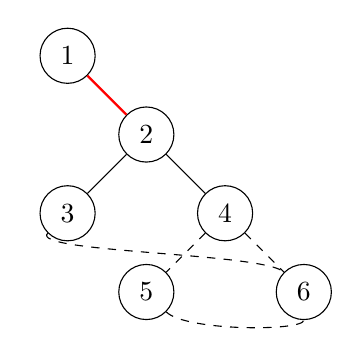
\begin{tikzpicture}[every node/.style={circle, draw, minimum size=0.7cm, inner sep=0pt}]
    \node (1) at (0,2) {1};
    \node (2) at (1,1) {2};
    \node (3) at (0,0) {3};
    \node (4) at (2,0) {4};
    \node (5) at (1,-1) {5};
    \node (6) at (3,-1) {6};

    \draw[red, thick] (1) -- (2);
    \draw (2) -- (3);
    \draw (2) -- (4);
    \draw[dashed] (4) -- (5);
    \draw[dashed] (4) -- (6);
    \draw[dashed] (3) .. controls (-0.5,-0.5) and (2.5,-0.5) .. (6); % thêm cạnh (3,6)
    \draw[dashed] (5) .. controls (1.5,-1.5) and (3,-1.5) .. (6); % thêm cạnh (5,6)
\end{tikzpicture}
\end{center}

Tuy nhiên, có một trường hợp cần chú ý: cạnh thêm vào có thể đã có sẵn trong đồ thị. Khi đó, ta cần tìm cạnh cầu trong một đa đồ thị, ta sẽ phải đánh dấu nếu cạnh đó đã sử dụng. \\

Để đánh dấu, ta có thể nén $id(u, v) = \min(u, v) \times 2\mathrm{e}5 + \max(u, v)$, lưu vào hashmap để truy vấn kiểm tra nhanh (tạm gọi là \texttt{edge\_cnt}). Sau đó kiểm tra cầu của đồ thị, nếu $edge\_cnt[id(u, v)] == 1$ thì đó là cầu.

\begin{lstlisting}[language=C++, caption={Cài đặt}]
#include <bits/stdc++.h>
#define int long long
#define endl "\n"
using namespace std;
const int MAXN = 2e5;
vector<int> adj[200005];
unordered_map<int, int> edge_cnt;
int n;
int low[MAXN + 5] = {0}, num[MAXN + 5] = {0};
int bridge = 0, timeDfs = 0;

int id(int a, int b) {
    return min(a, b) * MAXN + max(a,b);
}
void dfs(int u, int parent) {
    low[u] = num[u] = ++timeDfs;

    for (auto v : adj[u]) {
        if (v == parent) continue;
        if (num[v] == 0) {
            dfs(v, u);
            low[u] = min(low[v], low[u]);
            int a = u, b = v;
            if (low[v] > num[u] && edge_cnt[id(a,b)] == 1) {
                bridge++;
            }
        }
        else {
            low[u] = min(low[u], num[v]);
        }
    }
}
signed main() {
    ios_base::sync_with_stdio(0);
    cin.tie(0);
    cout.tie(0);
    cin >> n;
    for (int i = 1; i < n; i++) {
        int u, v; cin >> u >> v;
        adj[u].push_back(v);
        adj[v].push_back(u);
        edge_cnt[id(u,v)]++;
    }
    int m; cin >> m;
    for (int i = 1; i <= m; i++) {
        int u, v; cin >> u >> v;
        adj[u].push_back(v);
        adj[v].push_back(u);
        if (u > v) swap(u, v);
        if (edge_cnt.find(id(u,v)) != edge_cnt.end()) edge_cnt[id(u,v)]++;
    }
    for (int i = 1; i <= n; i++) {
        if (num[i] == 0) {
            dfs(i,i);
        }
    }
    cout << bridge;
    return 0;
}
\end{lstlisting}


\subsection{Thành phần liên thông mạnh (Strongly Connected Components)}

\begin{dinhnghia}
    
\end{dinhnghia}
 
\begin{itemize}
    \item Một đồ thị có hướng là liên thông mạnh nếu như từ một đỉnh bất kì luôn tồn tại ít nhất một đường đi đến bất kì đỉnh nào khác.
    \item Một thành phần liên thông mạnh của một đồ thị có hướng là một đồ thị con tối đại liên thông mạnh. Nếu mỗi thành phần liên thông mạnh được co lại thành một đỉnh, thì đồ thị sẽ trở thành một đồ thị có hướng không có chu trình.
    \item Thuật toán \textit{Kosaraju}, thuật toán \textit{Tarjan}, và thuật toán \textit{Gabow} đều có thể tìm các thành phần liên thông mạnh của một đồ thị cho trước trong thời gian tuyến tính. Tuy nhiên, các thuật toán của \textit{Tarjan} thường được sử dụng nhiều hơn do chúng chỉ cần thực hiện tìm kiếm theo chiều sâu một lần trong khi thuật toán của \textit{Kosaraju} cần hai lần.
\end{itemize}

\begin{figure}[h]
    \centering
    \includegraphics[width=0.4\textwidth]{img/b5/Depth-First-Search-Tree_img14.png}
    \caption{Minh họa thành phần liên thông mạnh (vùng xanh)}
\end{figure}

\subsubsection*{Một số định lý quan trọng}

\textbf{Định lý 1:} Nếu $a, b$ là hai đỉnh thuộc thành phần liên thông mạnh $C$ thì với mọi đường đi từ $a$ tới $b$ cũng như từ $b$ tới $a$, tất cả đỉnh trung gian trên đường đi đó đều phải thuộc $C$.

\textit{Chứng minh:} Nếu $a$ và $b$ là hai đỉnh thuộc $C$ thì tức là có một đường đi từ $a$ đến $b$ và một đường khác đi từ $b$ về $a$. Suy ra với một đỉnh $v$ nằm trên đường đi từ $a$ tới $b$ là ta tới được $v$, từ $b$ có đường tới $a$ nên $v$ cũng tới được $a$. Vậy $v$ nằm trong thành phần liên thông mạnh của $a$ tức là $v$ thuộc $C$. Trong tự vị mọi đỉnh nằm trên đường đi từ $b$ tới $a$.

\vspace{1em}
\textbf{Định lý 2:} Với một thành phần liên thông mạnh $C$ bất kỳ, tồn tại một đỉnh $r$ thuộc $C$ sao cho mọi đỉnh của $C$ đều thuộc cây con gốc $r$ trong cây \textit{DFS}.

\textit{Chứng minh:} Trước hết, nhắc lại một thành phần liên thông mạnh là một đồ thị con liên thông mạnh của đồ thị ban đầu thỏa mãn tính chất đại tại tức là không thể thêm một đỉnh nào vào mà vẫn giữ tính liên thông mạnh.\\
Trong số các đỉnh của $C$, chọn r là đỉnh được thăm đầu tiên khi thực hiện tìm kiếm theo chiều sâu. Ta sẽ chứng minh C nằm toàn bộ trong nhánh \textit{DFS} gốc $r$.\\
Thật vậy, với mọi đỉnh $v$ bất kỳ của $C$, có liên thông mạnh nên phải tồn tại một đường đi từ $r$ tới $v$: $(r = x_1, x_2, \dots, x_t = v)$.\\
Từ định lý 1, tất cả các đỉnh $x_1, x_2, \dots, x_t$ đều thuộc $C$ nên chúng sẽ phải thăm sau đỉnh $r$. Khi thủ tục \textit{DFS(r)} được gọi thì tất cả các đỉnh $x_1, x_2, \dots, x_t$ đều chưa thăm; như vậy thủ tục \textit{DFS(r)} sẽ liệt kê tất cả những đỉnh chưa thăm đến được từ r bằng cách xây dựng nhánh gốc r của cây \textit{DFS}, nên các đỉnh $x_1, x_2, \dots, x_t = v$ sẽ thuộc nhánh gốc r của cây \textit{DFS}. Bởi chọn r là đỉnh bất kỳ trong C nên ta có điều phải chứng minh.

Đỉnh $r$ trong chứng minh định lý - đỉnh thăm trước tất cả các đỉnh khác trong $C$ - gọi là chốt của thành phần C. Mỗi thành phần liên thông mạnh chỉ có một hoặc một vài chốt. Xét vị trí tương đối giữa các chốt trên cây \textit{DFS}, chốt của một thành phần liên thông mạnh là đỉnh nằm cao nhất so với các đỉnh khác thuộc thành phần đó, nói cách khác: là tiến đầu tiên để đi vào thành phần liên thông mạnh đó.

\vspace{1em}
\textbf{Định lý 3:} Luôn tìm được đỉnh chốt a thỏa mãn: Quá trình tìm kiếm theo chiều sâu bắt đầu từ a không thăm được bất kỳ một chốt nào khác. (Tức là nhánh \textit{DFS} gốc a không chứa một chốt nào nào ngoài a) chẳng hạn ta chọn a là chốt được thăm sau cùng trong một dãy chuyên về quy hoạch cho các chốt để thăm sau tất cả các chốt khác. Với chốt a như vậy thì các đỉnh thuộc nhánh \textit{DFS} gốc a chính là thành phần liên thông mạnh chứa a.

\textit{Chứng minh:} Với mọi đỉnh $v$ nằm trong nhánh \textit{DFS} gốc a, a là chốt của thành phần liên thông mạnh chứa v. Ta sẽ chứng minh bằng phản chứng. Nếu tồn tại một chốt $b \neq a$ phải nằm trong nhánh \textit{DFS} gốc a, thì nó sẽ mâu thuẫn với giả sử đã sắp xếp để a thăm sau các chốt khác. Vậy vẹn toàn trong nhánh \textit{DFS} gốc a và nhánh \textit{DFS} gốc a. Giả sử chứng rằng a khác b thì sẽ có hai trường hợp xảy ra.

\textbf{Trường hợp 1:} Nhánh \textit{DFS} gốc a chứa nhánh \textit{DFS} gốc b, có nghĩa là thủ tục \textit{DFS(b)} sẽ tới thủ tục \textit{DFS(a)} gọi tới, điều này mâu thuẫn với giả thiết rằng a là chốt mà quá trình tìm kiếm theo chiều sâu bắt đầu từ a không thăm một chốt nào khác.

\textbf{Trường hợp 2:} Nhánh \textit{DFS} gốc a và nhánh \textit{DFS} gốc b có nghĩa là a nằm trên một mớn đường từ b tới v. Do b và v thuộc cùng một thành phần liên thông mạnh nên theo định lý 1, a cũng phải thuộc thành phần liên thông mạnh đó. Suy ra b và a cùng là chốt của thành phần liên thông mạnh này có hai chốt a và b. Điều này vô lý.

Trong nhánh \textit{DFS} gốc a toàn thành phần liên thông mạnh chứa a, mà trong nhánh \textit{DFS} gốc a, theo chứng minh trên ta lại có: Mọi thành phần \textit{DFS} gốc a nằm trong thành phần liên thông mạnh chứa a. Kết hợp lại được: Nhánh \textit{DFS} gốc a chính là thành phần liên thông mạnh chứa a.

\begin{baitap}
    \href{https://oj.vnoi.info/problem/tjalg}{Tìm TPLT mạnh}
\end{baitap}

Cho đồ thị $G(V, E)$ có hướng $N$ $(1\leq N \leq 10^4)$ đỉnh $M$ $(1 \leq M \leq 10^5)$ cung. Hãy đếm số thành phần liên thông mạnh.\\

\textbf{Input}

Dòng đầu tiên là $M$, $N$.

$M$ dòng tiếp theo gồm 2 số nguyên $u, v$ mô tả một cung của $G$.\\

\textbf{Output} \\

Gồm một dòng duy nhất là số TPLT mạnh.\\

\textbf{Ví dụ}

\paragraph{Input}
\begin{lstlisting}
3 2
1 2
2 3
\end{lstlisting}

\paragraph{Output}
\begin{lstlisting}
3
\end{lstlisting}

\textbf{Thuật toán Tarjan}

\begin{figure}[h]
    \centering
    \includegraphics[width=0.6\textwidth]{img/b5/Depth-First-Search-Tree_img15.png}
\end{figure}

\textbf{Thuật toán Tarjan được xây dựng dựa trên các dữ kiện sau:}
\begin{itemize}
    \item Tìm kiếm \textit{DFS} tạo ra cây/rừng \textit{DFS}.
    \item Các thành phần liên thông mạnh tạo thành các cây con của cây \textit{DFS}.
    \item Nếu ta có thể tìm được đỉnh gốc của các cây con như vậy, ta có thể in/lưu trữ tất cả các nút trong cây con đó (bao gồm cả đỉnh gốc) và đó sẽ là một thành phần liên thông mạnh (\textit{Strongly Connected Components - SCC}).
    \item Không có cung ngược từ \textit{SCC} này sang \textit{SCC} khác (Có thể có các cung chéo, nhưng các cung chéo sẽ không được sử dụng trong khi xử lý đồ thị).
\end{itemize}

\textbf{Ý tưởng}
\begin{itemize}
    \item \textbf{Nhận xét:} Xét cây con gốc $u$ trong cây \textit{DFS}. Gọi tập hợp các đỉnh thuộc cây con gốc $u$ là $A$, tập hợp các đỉnh không thuộc cây con gốc $u$ là $B$. Nếu tồn tại 1 đỉnh $x$ thuộc $A$ tới được 1 đỉnh $y$ thuộc $B$ thì phải có thứ tự thăm sớm hơn $u$. Vì nếu $y$ được thăm sau $u$ ta có thể duyệt từ $u$ qua $x$ tới $y$ khi đó $y$ sẽ trở thành con của $u$.
    \item Đầu tiên ta thực hiện \textit{DFS} kết hợp tính mảng \texttt{low[]}, \texttt{num[]} như đã trình bày ở trên. Song song với việc này, khi duyệt tới đỉnh $u$ ta sẽ thực hiện đẩy $u$ vào \textit{stack}.
    \item Khi đã duyệt xong đỉnh $u$ (sau khi duyệt hết toàn bộ các đỉnh trong cây \textit{DFS} gốc $u$), nếu $num[u] = low[u]$ thì đây chính là đỉnh có thứ tự thăm sớm nhất của một thành phần liên thông mạnh.
    \item Khi đó ta sẽ loại bỏ tất cả các đỉnh trong thành phần liên thông mạnh này ra khỏi đồ thị và các đỉnh này là các đỉnh đang nằm trên $u$ trong \textit{stack} hiện tại vì các đỉnh này chính là các đỉnh nằm con gốc $u$ trong cây \textit{DFS} do các nút được đẩy vào \textit{stack} theo thứ tự thăm.
    \item Mặt khác, giả sử ta có đỉnh $x$ thuộc cây con gốc $u$ và $x$ thuộc thành phần liên thông mạnh không chứa $u$ có đỉnh có thứ tự thăm sớm nhất là $y$, để thấy $y$ phải là con của $u$ và nên thôi duyệt đỉnh $y$ sớm hơn $u$ chứng tỏ $y$ và thành phần liên thông mạnh chứa nó sẽ bị loại bỏ trước đó không còn trong \textit{stack} nữa (nếu còn thì ở đó vì ta đang xét mọi đỉnh trong cây con gốc $u$ chưa được xác định nằm trong thành phần liên thông mạnh nào trong các con gốc $u$).
    \item Ta sẽ đánh dấu tất cả các đỉnh thuộc thành phần liên thông mạnh bằng 1 mảng để sau này không xét lại đỉnh đấy nữa. Đồng thời, ta loại bỏ các đỉnh này ra khỏi \textit{stack} để không làm ảnh hưởng tới các đỉnh khác vẫn còn nằm trong đồ thị.
\end{itemize}

\subsection*{Cài đặt}

\textbf{Cấu trúc dữ liệu:}
\begin{itemize}
    \item Hằng số \texttt{maxN = 10000}
    \item Biến \texttt{timeDfs} -- Thứ tự \textit{DFS}
    \item Biến \texttt{scc} -- Số lượng thành phần liên thông mạnh
    \item Mảng \texttt{low[]}, \texttt{num[]}
    \item Mảng \texttt{deleted[]} -- Đánh dấu các đỉnh đã bị xóa
    \item Vector \texttt{adj[]} -- Danh sách cạnh kề của mỗi đỉnh
    \item Ngăn xếp \texttt{st} -- Lưu lại các đỉnh trong thành phần liên thông mạnh
\end{itemize}

\begin{lstlisting}[language=C++]
#include <bits/stdc++.h>
#define int long long
#define endl "\n"
using namespace std;
vector<int> adj[10005];
int n, m, timeDfs = 0;
const int MAXN = 1e4;
stack<int> st;
vector<bool> deleted(MAXN + 5, false);
vector<int> num(MAXN + 5, 0), low(MAXN + 5, 0);
int scc = 0;
void dfs(int u) {
    st.push(u);
    num[u] = low[u] = ++timeDfs;
    for (auto v : adj[u]) {
        if (num[v] == 0) {
            dfs(v);
            low[u] = min(low[u], low[v]);
        }
        else {
            if (deleted[v] == false) low[u] = min(low[u], num[v]);
        }
    }
    if (low[u] == num[u]) {
        int cur;
        scc++;
        do {
        cur = st.top();
        deleted[cur] = true;
        st.pop();
        } while (cur != u);
    }
}

signed main() {
    cin >> n >> m;
    for (int i = 1; i <= m; i++) {
        int u, v; cin >> u >> v;
        adj[u].push_back(v);
    }    
    for (int i = 1; i <= n; i++) {
        if (num[i] == 0) {
            dfs(i);
        }
    }
    cout << scc;
}
\end{lstlisting}

%---------------------------%
\begin{baitap}
    \href{https://oj.vnoi.info/problem/message}{Truyền tin}
\end{baitap}

Một lớp gồm $N$ học sinh, mỗi học sinh cho biết những bạn mà học sinh đó có thể liên lạc được (chú ý liên lạc này là liên lạc một chiều: $u$ có thể gửi tin tới $v$ nhưng $v$ thì chưa chắc đã có thể gửi tin tới $u$).

Thầy chủ nhiệm đang có một thông tin rất quan trọng cần thông báo tới tất cả các học sinh. Để tiết kiệm thời gian, thầy chỉ nhắn tin tới một số học sinh rồi sau đó nhờ các học sinh này nhắn lại cho tất cả các bạn mà các học sinh đó có thể liên lạc được, và cứ lần lượt như thế làm sao cho tất cả các học sinh trong lớp đều nhận được tin.

Hãy tìm một số ít nhất các học sinh mà thầy chủ nhiệm cần nhắn.

\textbf{Input}
\begin{itemize}
    \item Dòng đầu là $N, M$ ($N \leq 800$, $M$ là số lượng liên lạc 1 chiều)
    \item Một số dòng tiếp theo mỗi dòng gồm 2 số $u, v$ cho biết học sinh $u$ có thể gửi tin tới học sinh $v$
\end{itemize}

\textbf{Output} 
\begin{itemize}
    \item Gồm 1 dòng ghi số học sinh cần thầy nhắn tin.
\end{itemize}


\textbf{Ví dụ}

\paragraph{Input}
\begin{lstlisting}
12 15
1 3
3 6
6 1
6 8
8 12
12 9
9 6
2 4
4 5
5 2
4 6
7 10
10 11
11 7
10 9
\end{lstlisting}

\paragraph{Output}
\begin{lstlisting}
2
\end{lstlisting}

\subsubsection*{Phân tích}

Đầu tiên, ta gom các đỉnh thành các \textbf{thành phần liên thông mạnh} (SCC) -- tức là xác định những nhóm đỉnh mà trong đó, bất kỳ bạn nào nhận được tin cũng có thể truyền tin cho tất cả các bạn còn lại trong cùng nhóm đó. Việc gom nhóm này giúp rút gọn bài toán: với mỗi SCC, chỉ cần một học sinh trong nhóm nhận tin thì cả nhóm sẽ nhận được tin.

Tiếp theo, ta xây dựng \textbf{đồ thị rút gọn} giữa các SCC: mỗi nhóm là một đỉnh, có cung nối từ nhóm này sang nhóm khác nếu có ít nhất một học sinh trong nhóm đầu liên lạc được với học sinh trong nhóm sau. Lúc này, tin chỉ có thể lan truyền từ SCC này sang SCC khác theo các cung của đồ thị rút gọn.

Bây giờ, chỉ cần xét \textbf{bậc vào} (\textit{in-degree}) của mỗi SCC trong đồ thị rút gọn:
\begin{itemize}
    \item Những nhóm nào có bậc vào lớn hơn 0 sẽ nhận được tin từ các nhóm khác.
    \item Ngược lại, các nhóm không có bậc vào (in-degree bằng 0) là những nhóm không nhận được tin từ bất kỳ nhóm nào khác. Vì vậy, thầy chủ nhiệm bắt buộc phải gửi tin trực tiếp cho ít nhất một học sinh ở mỗi nhóm này, để tin có thể lan truyền tiếp đi.
\end{itemize}

Tóm lại, đáp số là \textbf{số lượng SCC có bậc vào bằng 0} trong đồ thị rút gọn. Đây cũng chính là số học sinh ít nhất mà thầy cần nhắn tin ban đầu.

\begin{figure}[h]
    \centering
    \includegraphics[width=0.6\textwidth]{img/b5/message.png}
    \caption{Đồ thị ban đầu và Đồ thị sau khi gom nhóm theo SCC}
\end{figure}

\begin{lstlisting}[language=C++, caption={Cài đặt}]
#include <bits/stdc++.h>
#define int long long
#define endl "\n"
using namespace std;
vector<int> adj[805];
const int MAXN = 800;
int n, m, timeDfs = 0;
vector<int> num(MAXN + 5, 0), low(MAXN + 5, 0);
vector<bool> deleted(MAXN + 5, false);
stack<int> st;
int scc = 0;
vector<int> comp(MAXN + 5);

void dfs(int u) {
    st.push(u);
    num[u] = low[u] = ++timeDfs;
    for (auto v : adj[u]) {
        if (deleted[v]) continue;
        if (num[v] == 0) {
            dfs(v);
            low[u] = min(low[v], low[u]);
        }
        else {
            low[u] = min(low[u], num[v]);
        }
    }    
    if (num[u] == low[u]) {
        int cur;
        do {
            cur = st.top(); st.pop();
            deleted[cur] = true;
            comp[cur] = scc;
        } while (cur != u);
        scc++;
    }
}
signed main() {
    cin >> n >> m;
    for (int i = 1; i <= m; i++) {
        int u, v; cin >> u >> v;
        adj[u].push_back(v);
    }
    for (int i = 1; i <= n; i++) {
        if (num[i] == 0) dfs(i);
    }
    vector<int> in_deg(scc, 0);
    for (int u = 1; u <= n; u++) {
        for (auto v : adj[u]) {
            if (comp[u] != comp[v]) {
                in_deg[comp[v]]++;
            }
        }
    }
    int ans = 0;
    for (int i = 0; i < scc; i++) {
        if (in_deg[i] == 0) {
            ans++;
        }
    }
    cout << ans;
}
\end{lstlisting}

%---------------------------%
\begin{baitap}
    \href{https://oj.vnoi.info/problem/nkonearc}{VOI 06 Bài 5 - Mạng máy tính}
\end{baitap}

Một hệ thống $n$ máy tính (các máy tính được đánh số từ $1$ đến $n$) được nối lại thành một mạng bởi $m$ kênh nối, mỗi kênh nối hai máy nào đó và cho phép ta truyền tin một chiều từ máy này đến máy kia. Giả sử $s$ và $t$ là 2 máy tính trong mạng. Ta gọi đường truyền từ máy $s$ đến máy $t$ là một dãy các máy tính và các kênh nối chúng có dạng:
\[
s = u_1, e_1, u_2, \ldots, u_i, e_i, u_{i+1}, \ldots, u_{k-1}, e_{k-1}, u_k = t
\]
trong đó $u_1, u_2, \ldots, u_k$ là các máy tính trong mạng, $e_i$ là kênh truyền tin từ máy $u_i$ đến máy $u_{i+1}$ ($i = 1, 2, \ldots, k-1$).

Mạng máy tính được gọi là \textbf{thông suốt} nếu như đối với hai máy $u, v$ bất kỳ ta luôn có đường truyền tin từ $u$ đến $v$ và đường truyền tin từ $v$ đến $u$. Mạng máy tính được gọi là \textbf{hầu như thông suốt} nếu đối với hai máy $u, v$ bất kỳ, hoặc là có đường truyền từ $u$ đến $v$, hoặc là có đường truyền từ $v$ đến $u$.

Biết rằng mạng máy tính đã cho là hầu như thông suốt nhưng không thông suốt.

Yêu cầu: hãy xác định xem có thể bổ sung đúng một kênh truyền tin để biến mạng đã cho trở thành thông suốt được không?

\textbf{Input}
\begin{itemize}
    \item Dòng đầu tiên ghi 2 số nguyên $n$ và $m$.
    \item Dòng thứ $i$ trong số $m$ dòng tiếp theo mô tả kênh nối thứ $i$ bao gồm 2 số nguyên dương $u_i$ và $v_i$ cho biết kênh nối thứ $i$ cho phép truyền tin từ máy $u_i$ đến máy $v_i$, $i = 1, 2, \ldots, m$.
\end{itemize}
Các số trên cùng một dòng được ghi cách nhau bởi dấu cách.

\textbf{Output}
\begin{itemize}
    \item Dòng đầu tiên ghi 'YES' nếu câu trả lời là khẳng định, ghi 'NO' nếu câu trả lời là phủ định.
    \item Nếu câu trả lời là khẳng định thì ghi ra hai số nguyên dương $u, v$ cách nhau bởi dấu cách cho biết cần bổ sung kênh truyền tin từ máy $u$ đến máy $v$ để biến mạng thành thông suốt.
\end{itemize}

\textbf{Giới hạn}

Trong tất cả các test, $n \leq 2000, m \leq 30000$.

\textbf{Ví dụ}

\paragraph{Input}
\begin{lstlisting}
3 2
1 2
2 3
\end{lstlisting}

\paragraph{Output}
\begin{lstlisting}
YES
3 1
\end{lstlisting}

\textbf{Minh họa ví dụ, cạnh đỏ là cạnh cần thêm vào để đồ thị thông suốt}

\begin{center}
    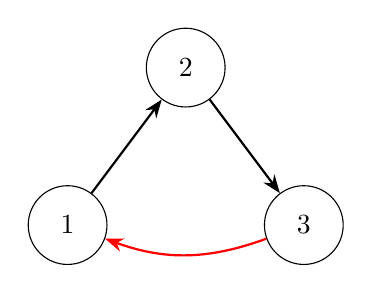
\begin{tikzpicture}[every node/.style={circle,draw,minimum size=1cm,inner sep=0pt}, 
        >=Stealth, node distance=2.2cm]
        % Các đỉnh
        \node (1) at (0,0) {1};
        \node (2) at (1.5,2) {2};
        \node (3) at (3,0) {3};

        % Các cạnh gốc
        \draw[->, thick] (1) -- (2);
        \draw[->, thick] (2) -- (3);

        % Cạnh thêm (đỏ)
        \draw[->, thick, red] (3) to [bend left=20] (1);
    \end{tikzpicture}
\end{center}

\textbf{Phân tích}

Đầu tiên, ta gom các đỉnh của đồ thị gốc thành các SCC. Kết quả thu được là một đồ thị rút gọn, trong đó mỗi SCC được coi là một siêu-đỉnh. Bài toán bổ sung đúng một cạnh để đồ thị trở thành liên thông mạnh tương đương với việc bổ sung một cạnh vào đồ thị rút gọn sao cho toàn bộ các SCC hợp thành một chu trình duy nhất.

Để làm được điều này, ta nhận thấy: trong đồ thị rút gọn, một siêu-đỉnh $u$ là ứng viên đầu nối nếu nó có bậc ra bằng 0 (deg\_out$[u]=0$) và bậc vào lớn hơn 0 (deg\_in$[u] > 0$); ngược lại, một siêu-đỉnh $v$ là ứng viên đuôi nối nếu nó có bậc vào bằng 0 (deg\_in$[v]=0$) và bậc ra lớn hơn 0 (deg\_out$[v] > 0$).

Khi đó, chỉ cần nối một cạnh từ một siêu-đỉnh thuộc đồ thị rút gọn có bậc ra bằng 0 đến một siêu-đỉnh thuộc đồ thị rút gọn có bậc vào bằng 0 là đủ để biến đồ thị thành liên thông mạnh.

%\begin{multicols}{2}

\begin{lstlisting}[language=C++, caption={Cài đặt}]
#include <bits/stdc++.h>
#define int long long
#define endl "\n"
using namespace std;
vector<int> adj[2005];
const int MAXN = 2000;
int n, m, timeDfs = 0;
stack<int> st;
vector<bool> deleted(MAXN + 5, false);
vector<int> deg_in(MAXN + 5, 0), deg_out(MAXN + 5, 0);
vector<int> num(MAXN + 5, 0), low(MAXN + 5, 0);
vector<int> comp(MAXN + 5, 0);
int scc = 0;

void dfs(int u) {
    num[u] = low[u] = ++timeDfs;
    st.push(u);
    for (auto v : adj[u]) {
        if (deleted[v] == true) continue;
        if (num[v] == 0) {
            dfs(v);
            low[u] = min(low[u], low[v]);
        }
        else {
            low[u] = min(low[u], num[v]);
        }
    }

    if (low[u] == num[u]) {
        int v;
        do {
            v = st.top(); st.pop();
            deleted[v] = true;
            comp[v] = scc;
        } while (v != u);
        scc++;
    }
}
signed main() {
    cin >> n >> m;
    for (int i = 1; i <= m; i++) {
        int u, v; cin >> u >> v;
        adj[u].push_back(v);
    }
    for (int i = 1; i <= n; i++) {
        if (num[i] == 0) dfs(i);
    }
    for (int u = 1; u <= n; u++) {
        for (auto v : adj[u]) {
            if (comp[u] != comp[v]) {
                deg_out[comp[u]]++;
                deg_in[comp[v]]++;
            }
        }
    }

    int u = -1, v = -1;
    for (int i = 0; i < scc; i++) {
        if (deg_out[i] == 0 && deg_in[i] > 0) {
            if (u != -1) {
                cout << "NO";
                return 0;
            }
            u = i;
        }
        if (deg_in[i] == 0 && deg_out[i] > 0) {
            if (v != -1) {
                cout << "NO";
                return 0;
            }
            v = i;
        }
    }
    bool ok1 = false, ok2 = false;
    for (int i = 1; i <= n; i++) {
        if (comp[i] == u && ok1 == false) {
            u = i;
            ok1 = true;
        }
        if (comp[i] == v && ok2 == false) {
            v = i;
            ok2 = true;
        }
    }
    cout << "YES\n" << u << " " << v;
}
\end{lstlisting}
%\end{multicols}


%---------------------------%
\begin{baitap}
    \href{https://cses.fi/problemset/task/1686}{Coin Collector}
\end{baitap}

Một trò chơi gồm $n$ căn phòng và $m$ đường hầm nối giữa chúng. Mỗi phòng có một số lượng xu nhất định. Hỏi số lượng xu lớn nhất bạn có thể thu thập được khi di chuyển qua các đường hầm, trong trường hợp bạn được phép tự do chọn phòng bắt đầu và phòng kết thúc?

\textbf{Input}
\begin{itemize}
    \item Dòng đầu tiên gồm hai số nguyên $n$ và $m$: số lượng phòng và số lượng đường hầm. Các phòng được đánh số từ $1, 2, \ldots, n$.
    \item Dòng tiếp theo gồm $n$ số nguyên $k_1, k_2, \ldots, k_n$: số lượng xu ở mỗi phòng.
    \item Cuối cùng là $m$ dòng mô tả các đường hầm. Mỗi dòng gồm hai số nguyên $a$ và $b$, nghĩa là có một đường hầm một chiều từ phòng $a$ tới phòng $b$.
\end{itemize}

\textbf{Output}
\begin{itemize}
    \item In ra một số nguyên: số lượng xu lớn nhất bạn có thể thu thập được.
\end{itemize}

\textbf{Ràng buộc}
\begin{itemize}
    \item $1 \leq n \leq 10^5$
    \item $1 \leq m \leq 2 \cdot 10^5$
    \item $1 \leq k_i \leq 10^9$
    \item $1 \leq a, b \leq n$
\end{itemize}

\textbf{Ví dụ}

\paragraph{Input}
\begin{lstlisting}
4 4
4 5 2 7
1 2
2 1
1 3
2 4
\end{lstlisting}

\paragraph{Output}
\begin{lstlisting}
16
\end{lstlisting}

\textbf{Phân tích}

Đầu tiên, ta gom các đỉnh của đồ thị gốc thành các SCC. Kết quả thu được là một đồ thị rút gọn, trong đó mỗi SCC được coi là một siêu-đỉnh, và giữa hai siêu-đỉnh $u$ và $v$ có cung hướng nếu tồn tại ít nhất một cạnh hướng từ một đỉnh trong SCC tương ứng với $u$ sang một đỉnh trong SCC tương ứng với $v$.  

Mỗi siêu-đỉnh $u$ mang trọng số bằng tổng số xu ở tất cả các phòng thuộc SCC đó. Do đồ thị rút gọn luôn là một đồ thị có hướng không chu trình (DAG), bài toán thu gọn thành việc tìm đường đi có tổng trọng số lớn nhất trên DAG này.

Gọi $\mathrm{dp}[u]$ là số xu lớn nhất có thể thu thập được khi xuất phát từ siêu-đỉnh $u$. Ta khởi tạo
\[
\mathrm{dp}[u] \;=\; \text{cost}[u],
\]
với \texttt{cost[u]} là trọng số (tổng xu) của SCC tương ứng. Sau đó, duyệt các cung $u \to v$ trên DAG (Code bên dưới thực hiện đệ quy có nhớ, có thể tối ưu hơn (hoặc không) bằng sắp xếp tô-pô), ta cập nhật
\[
\mathrm{dp}[u] \;=\; \max\bigl(\mathrm{dp}[u],\;\text{cost}[u] + \mathrm{dp}[v]\bigr).
\]
Cuối cùng, đáp án là
\[
\max_{u}\,\mathrm{dp}[u],
\]
tức tổng xu lớn nhất có thể thu thập khi được phép chọn tự do phòng bắt đầu (tương đương siêu-đỉnh $u$ khởi hành).  

\begin{lstlisting}[language=C++, caption={Cài đặt}]
#include <bits/stdc++.h>
#define int long long
#define endl "\n"
using namespace std;
int n, m, timeDfs = 0, scc = 0;
const int MAXN = 1e5;
vector<int> k, adj[100005], num(MAXN + 5, 0), low(MAXN + 5, 0), comp(MAXN + 5, 0);
vector<bool> deleted(MAXN + 5, false);
vector<int> cost(MAXN + 5, 0), dp;
vector<vector<int>> bigNode;
stack<int> st;
void dfs(int u) {
    st.push(u);
    num[u] = low[u] = ++timeDfs;
    for (auto v : adj[u]) {
        if (deleted[v] == true) continue;
        if (num[v] == 0) {
            dfs(v);
            low[u] = min(low[u], low[v]);
        } else {
            low[u] = min(low[u], num[v]);
        }
    }
    if (num[u] == low[u]) {
        int v;
        do {
            v = st.top(); st.pop();
            deleted[v] = true;
            comp[v] = scc;
            cost[scc] += k[v];
        } while (v != u);
        scc++;
    }
}

void findCost(int u) {
    if (dp[u] != -1) return;
    dp[u] = cost[u];
    for (auto v : bigNode[u]) {
        findCost(v);
        dp[u] = max(dp[u], dp[v] + cost[u]);
    }
}

signed main() {
    cin >> n >> m;
    k.resize(n + 1);
    for (int i = 1; i <= n; i++) {
        cin >> k[i];
    }
    for (int i = 1; i <= m; i++) {
        int u, v; cin >> u >> v;
        adj[u].push_back(v);
    }
    for (int i = 1; i <= n; i++) {
        if (num[i] == 0) dfs(i);
    }
    bigNode.resize(scc);
    dp.resize(scc, -1);
    for (int u = 1; u <= n; u++) {
        for (auto v : adj[u]) {
            if (comp[u] != comp[v]) {
                bigNode[comp[u]].push_back(comp[v]);
            }
        }
    }
    for (int i = 0; i < scc; i++) {
        if (dp[i] == -1) {
            findCost(i);
        }
    }
    cout << *max_element(dp.begin(), dp.end());   
}
\end{lstlisting}

\subsection{Thuật toán BFS}

Nội dung bài chủ yếu tham khảo/copy từ [VNOI WIKI]: \url{https://wiki.vnoi.info/algo/graph-theory/breadth-first-search.md}


\subsubsection{Thuật toán duyệt đồ thị ưu tiên chiều rộng}

Thuật toán \textbf{duyệt đồ thị ưu tiên chiều rộng} (\textit{Breadth-first search} - BFS) là một trong những thuật toán tìm kiếm cơ bản và thiết yếu trên đồ thị. Trong đó, những đỉnh nào gần đỉnh xuất phát hơn sẽ \textbf{được duyệt trước}.

Ứng dụng của \textit{BFS} có thể giúp ta giải quyết tốt một số bài toán trong thời gian và không gian \textbf{tối thiểu}. Đặc biệt là bài toán tìm kiếm đường đi ngắn nhất từ một đỉnh gốc tới tất cả các đỉnh khác. Trong đồ thị không có trọng số hoặc tất cả trọng số bằng nhau, thuật toán sẽ luôn trả ra đường đi ngắn nhất có thể. Ngoài ra, thuật toán này còn được dùng để tìm các thành phần liên thông của đồ thị, hoặc kiểm tra đồ thị hai phía, \ldots

\begin{figure}[h]
    \centering
    \includegraphics[width=0.4\textwidth]{img/b6/breadth-first-search_img1.png}
    \caption{Thứ tự thăm các đỉnh của BFS}
\end{figure}

\subsubsection{Ý tưởng}

Với đồ thị không trọng số và đỉnh nguồn $s$. Đồ thị này có thể là đồ thị có hướng hoặc vô hướng, điều đó \textbf{không quan trọng} đối với thuật toán. 

Có thể hiểu thuật toán như một ngọn lửa lan rộng trên đồ thị:

\begin{itemize}
    \item Ở bước thứ $0$, chỉ có đỉnh nguồn $s$ đang cháy.
    \item Ở mỗi bước tiếp theo, ngọn lửa đang cháy ở mỗi đỉnh lại lan sang tất cả các đỉnh kề với nó.
\end{itemize}

Trong mỗi lần lặp của thuật toán, ``vòng lửa'' lại lan rộng ra theo chiều rộng. Những đỉnh nào gần $s$ hơn sẽ bùng cháy trước.

Chính xác hơn, thuật toán có thể được mô tả như sau:
\begin{itemize}
    \item Đầu tiên ta thăm đỉnh nguồn $s$.
    \item Việc thăm đỉnh $s$ sẽ phát sinh thứ tự thăm các đỉnh $(u_1, u_2, \ldots, u_p)$ kề với $s$ (những đỉnh gần $s$ nhất). Tiếp theo, ta thăm đỉnh $u_1$, khi thăm đỉnh $u_1$ sẽ lại phát sinh yêu cầu thăm những đỉnh $(v_1, v_2, \ldots, v_q)$ kề với $u_1$. Nhưng rõ ràng những đỉnh $v$ này ``xa'' $s$ hơn những đỉnh $u$ nên chúng chỉ được thăm khi tất cả những đỉnh $u$ đều đã được thăm. Tức là thứ tự thăm các đỉnh sẽ là: $s, u_1, u_2, \ldots, u_p, v_1, v_2, \ldots, v_q, \ldots$
\end{itemize}

\begin{figure}[h]
    \centering
    \includegraphics[width=0.5\textwidth]{img/b6/breadth-first-search_img2.png}
\end{figure}

Thuật toán tìm kiếm theo chiều rộng sử dụng một danh sách để chứa những đỉnh đang ``chờ'' thăm. Tại mỗi bước, ta thăm một đỉnh đầu danh sách, loại nó ra khỏi danh sách và cho những đỉnh kề với nó chưa được thăm xếp hàng vào cuối danh sách. Thuật toán sẽ kết thúc khi danh sách rỗng.

\subsubsection{Thuật toán}

Thuật toán sử dụng một cấu trúc dữ liệu hàng đợi (\textit{queue}) để chứa các đỉnh sẽ được duyệt theo thứ tự ưu tiên chiều rộng.

\textbf{Bước 1: Khởi tạo}
\begin{itemize}
    \item Các đỉnh đều ở trạng thái chưa được đánh dấu. Ngoại trừ đỉnh nguồn $s$ đã được đánh dấu.
    \item Một hàng đợi ban đầu chỉ chứa 1 phần tử là $s$.
\end{itemize}

\textbf{Bước 2: Lặp lại các bước sau cho đến khi hàng đợi rỗng:}
\begin{itemize}
    \item Lấy đỉnh $u$ ra khỏi hàng đợi.
    \item Xét tất cả những đỉnh $v$ kề với $u$ mà chưa được đánh dấu, với mỗi đỉnh $v$ đó:
    \begin{itemize}
        \item Đánh dấu $v$ đã thăm.
        \item Lưu lại vết đường đi từ $u$ đến $v$.
        \item Đẩy $v$ vào trong hàng đợi (đỉnh $v$ sẽ chờ được duyệt tại những bước sau).
    \end{itemize}
\end{itemize}

\textbf{Bước 3:} Truy vết tìm đường đi.

\subsubsection{Mô tả}

\begin{itemize}
    \item Xét đồ thị sau đây, với đỉnh nguồn $s = 1$:
\end{itemize}

\begin{figure}[h]
    \centering
    \includegraphics[width=0.5\textwidth]{img/b6/breadth-first-search_img3.png}
\end{figure}
\begin{figure}[h]
    \centering
    \includegraphics[width=0.5\textwidth]{img/b6/breadth-first-search_img4.png}
\end{figure}

\subsubsection{Cài đặt}

\textbf{Cấu trúc dữ liệu:}
\begin{itemize}
    \item \texttt{n}: Số lượng đỉnh của đồ thị.
    \item \texttt{const int MAXN = 100005}: Kích thước tối đa cho các mảng.
    \item \texttt{vector<int> dist}: Mảng lưu khoảng cách (số bước) ngắn nhất từ đỉnh nguồn đến các đỉnh.
    \item \texttt{vector<int> parent}: Mảng lưu lại ``cha'' (đỉnh trước đó) trên đường đi ngắn nhất từ nguồn đến mỗi đỉnh.
    \item \texttt{vector<bool> visited}: Mảng đánh dấu các đỉnh đã được thăm.
    \item \texttt{vector<int> adj[MAXN]}: Danh sách kề (adjacency list) của mỗi đỉnh.
\end{itemize}

\begin{lstlisting}[language=C++, caption={Cài đặt}]
int n; 
const int MAXN = 100005;
vector<int> dist(MAXN, 0), parent(MAXN, -1);
vector<bool> visited(MAXN, false);
vector <int> adj[MAXN];

void bfs(int s) { 
    queue <int> q;
    q.push(s);
    visited[s] = true;
    while (q.empty() == false) {
        int u = q.front();
        q.pop();
        for (auto v : adj[u]) {
            if (visited[v] == false) {
                dist[v] = dist[u] + 1;
                parent[v] = u;
                visited[v] = true;
                q.push(v);
            }
        }
    }
}
\end{lstlisting}

\textbf{Truy vết:}
\begin{lstlisting}[language=C++, caption={Cài đặt truy vết đường đi từ đỉnh nguồn $s$ đến đỉnh $u$}]
if (visited[u] == false) {
    cout << "No path!";
} else {
    vector<int> path;
    for (int v = u; v != -1; v = parent[v])
        path.push_back(v);
    reverse(path.begin(), path.end());

    cout << "Path: ";
    for (auto v : path) cout << v << ' ';
}
\end{lstlisting}

\subsubsection{Các đặc tính của thuật toán}

Nếu sử dụng một ngăn xếp (\textit{stack}) thay vì hàng đợi (\textit{queue}) thì ta sẽ thu được \textbf{thứ tự duyệt đỉnh} của thuật toán \textbf{tìm kiếm theo chiều sâu} (\textit{Depth First Search} -- DFS). Đây chính là \textbf{phương pháp khử đệ quy} của DFS để cài đặt thuật toán trên các ngôn ngữ không cho phép đệ quy.

\textbf{Định lý:} Thuật toán \textit{BFS} cho ta độ dài đường đi ngắn nhất từ đỉnh nguồn tới mọi đỉnh (với khoảng cách tới đỉnh $u$ bằng $d[u]$).  
Trong thuật toán \textit{BFS}, nếu đỉnh $u$ xa đỉnh nguồn hơn đỉnh $v$, thì $u$ sẽ được thăm sau $v$.

\begin{itemize}
    \item \textbf{Chứng minh:} Trong \textit{BFS}, từ một đỉnh hiện tại, ta luôn đi thăm tất cả các đỉnh kề với nó trước, sau đó thăm tất cả các đỉnh cách nó một đỉnh, rồi các đỉnh cách nó hai đỉnh, v.v... Như vậy, nếu từ một đỉnh $u$ khi ta chạy \textit{BFS}, quãng đường đến đỉnh $v$ luôn là quãng đường đi qua ít cạnh nhất.
\end{itemize}

\subsubsection{Định lý Bắt tay (Handshaking lemma)}

\textbf{Định lý:} Trong một đồ thị bất kỳ, tổng số bậc của tất cả các đỉnh bằng \textbf{gấp đôi} số cạnh của đồ thị.

\textbf{Mô tả:} Cho đồ thị $G = (V, E)$ gồm $|V|$ đỉnh và $|E|$ cạnh. Khi đó, tổng tất cả các bậc của đỉnh trong $G$ bằng $2 \times |E|$.  
Với $\deg(v)$ là số bậc của đỉnh $v$, có:
\[
\sum_{v \in V} \deg(v) = 2 \times |E|
\]

\textbf{Ví dụ:} Cho đồ thị sau với $|V| = 8$ và $|E| = 7$:

\begin{figure}[h]   
    \centering
    \includegraphics[width=0.5\textwidth]{img/b6/breadth-first-search_img5.png}
\end{figure}

\[
\sum_{v \in V} \deg(v) = 2 \times |E| = 2 \times 7 = 14
\]

\textbf{Chứng minh:}  
Vì mỗi một cạnh nối với đúng hai đỉnh của đồ thị, nên một cạnh sẽ đóng góp $2$ đơn vị vào tổng số bậc của tất cả các đỉnh.

\textbf{Hệ quả:} Trong đồ thị, số lượng \textbf{đỉnh bậc lẻ} luôn là một số chẵn.

\textbf{Chứng minh:} Gọi $L$ và $C$ lần lượt là tập các đỉnh bậc lẻ và bậc chẵn của đồ thị $G=(V,E)$. Ta có:
\[
2 \times |E| = \sum_{v \in V} \deg(v) = \sum_{v \in C} \deg(v) + \sum_{v \in L} \deg(v)
\]
$2 \times |E|$ là số chẵn $\implies \sum_{v \in C} \deg(v)$ chẵn, $\sum_{v \in L} \deg(v)$ chẵn $\implies$ số phần tử của $L$ là chẵn.

\textbf{Nhận xét:}
\begin{itemize}
    \item Trong quá trình duyệt đồ thị được biểu diễn bằng \textbf{danh sách kề}, mỗi cạnh sẽ được duyệt chính xác hai lần đối với \textbf{đồ thị vô hướng} (vì mỗi cạnh sẽ được lưu trong 2 danh sách kề của 2 đỉnh). Còn đối với \textbf{đồ thị có hướng}, mọi cạnh của đồ thị chỉ được duyệt chính xác một lần.
\end{itemize}

\textbf{Tham khảo:} \href{https://en.wikipedia.org/wiki/Handshaking_lemma}{Handshaking\_lemma}

\subsubsection{Độ phức tạp thuật toán}

\paragraph{Độ phức tạp thời gian}

Gọi $|V|$ là số lượng đỉnh và $|E|$ là số lượng cạnh của đồ thị.

Trong quá trình \textit{BFS}, cách biểu diễn đồ thị có ảnh hưởng lớn tới chi phí về thời gian thực hiện giải thuật:

\begin{itemize}
    \item \textbf{Nếu đồ thị biểu diễn bằng danh sách kề} (\texttt{vector g[]}):

    \begin{itemize}
        \item Ta có thể thực hiện thuật toán này một cách tối ưu nhất về mặt thời gian nhờ khả năng duyệt qua các đỉnh kề của mỗi đỉnh một cách hiệu quả.
        \item Vì ta sử dụng mảng \texttt{visited[]} để ngăn việc đẩy một đỉnh vào hàng đợi nhiều lần nên mỗi đỉnh sẽ được thăm \textbf{chính xác một lần} duy nhất. Do đó, ta mất độ phức tạp thời gian $O(|V|)$ cho việc thăm các đỉnh.
        \item Bất cứ khi nào một đỉnh được thăm, mọi cạnh kề với nó đều được duyệt, với thời gian dành cho mỗi cạnh là $O(1)$. Từ nhận nhận xét của định lý Bắt tay (\textit{Handshaking lemma}), ta sẽ mất độ phức tạp thời gian $O(|E|)$ dành cho việc duyệt các cạnh.
        \item Nhìn chung, độ phức tạp thời gian của thuật toán là $O(|V| + |E|)$. Đây là cách cài đặt tối ưu nhất.
    \end{itemize}

    \item \textbf{Nếu như đồ thị được biểu diễn bằng ma trận kề:}
    \begin{itemize}
        \item Ta cũng sẽ mất độ phức tạp thời gian $O(|V|^2)$ cho việc thăm các đỉnh (giải thích tương tự như trên).
        \item Với mỗi đỉnh được thăm, ta phải duyệt qua toàn bộ các đỉnh của đồ thị để kiểm tra đỉnh kề với nó. Do đó, thuật toán sẽ mất độ phức tạp $O(|V|^2)$.
    \end{itemize}
\end{itemize}

\paragraph{Độ phức tạp không gian}
Tại mọi thời điểm, trong hàng đợi (\texttt{queue q}) có không quá $|V|$ phần tử. Do đó, độ phức tạp bộ nhớ là $O(|V|)$.

\subsection{Ứng dụng BFS để xác định thành phần liên thông}

\begin{baitap}    
    \href{https://lequydon.ntucoder.net/Problem/Details/4601}{BDFS - Đếm số thành phần liên thông}
\end{baitap}
Cho đơn đồ thị vô hướng gồm $n$ đỉnh và $m$ cạnh ($1 \leq n, m \leq 10^5$), các đỉnh được đánh số từ $1$ tới $n$. Tìm số \textbf{thành phần liên thông} của đồ thị.

\subsubsection{Ý tưởng}

Một đồ thị có thể liên thông hoặc không liên thông. Nếu đồ thị liên thông thì số thành phần liên thông của nó là $1$. Điều này tương đương với phép duyệt theo thủ tục \textit{BFS} được gọi đến đúng một lần. Nếu đồ thị không liên thông (số thành phần liên thông lớn hơn $1$), ta có thể tách chúng thành những \textbf{đồ thị con liên thông}. Điều này cũng có nghĩa là trong phép duyệt đồ thị, số thành phần liên thông của nó bằng số lần gọi tới thủ tục \textit{BFS}.

\subsubsection{Thuật toán}

Thuật toán ứng dụng \textit{BFS} để xác định thành phần liên thông:

\begin{itemize}
    \item \textbf{Bước 0:} Khởi tạo số lượng thành phần liên thông bằng $0$.
    \item \textbf{Bước 1:} Xuất phát từ một đỉnh chưa được đánh dấu của đồ thị. Ta đánh dấu đỉnh xuất phát, tăng số thành phần liên thông thêm $1$.
    \item \textbf{Bước 2:} Từ một đỉnh đã đánh dấu, đánh dấu tất cả các đỉnh $j$ kề với $i$ mà $j$ chưa được đánh dấu.
    \item \textbf{Bước 3:} Thực hiện bước 2 cho đến khi không còn đỉnh nào được nữa.
    \item \textbf{Bước 4:} Nếu số đỉnh chưa đánh dấu (mảng \texttt{visited} chưa đánh dấu) kết thúc thuật toán và trả về số thành phần liên thông, ngược lại quay về bước 1.
\end{itemize}

\begin{lstlisting}[language=C++, caption={Cài đặt, độ phức tạp $O(M + N)$}]
#include <bits/stdc++.h>
#define int long long
#define endl "\n"
using namespace std;

int n, m, componentNumber = 0; 
const int MAXN = 100005;
vector<bool> visited(MAXN, false);
vector <int> adj[MAXN];

void bfs(int s) { 
    queue <int> q;
    q.push(s);
    visited[s] = true;
    while (q.empty() == false) {
        int u = q.front();
        q.pop();
        for (auto v : adj[u]) {
            if (visited[v] == false) {
                dist[v] = dist[u] + 1;
                parent[v] = u;
                visited[v] = true;
                q.push(v);
            }
        }
    }
    componentNumber++;
}

signed main() {
    cin >> n >> m;
    for (int i = 1; i <= m; i++) {
        int u, v; cin >> u >> v;
        adj[u].push_back(v);
        adj[v].push_back(u);
    }
    for (int u = 1; u <= n; u++) {
        if (visited[u] == false) {
            bfs(u);
        }
    }
    cout << componentNumber;
}
\end{lstlisting}

\subsection{Ứng dụng BFS để tìm đường đi ngắn nhất trong đồ thị có trọng số 0 hoặc 1}

\begin{baitap}
    \href{https://site.ada.edu.az/~medv/acm/Docs%20Codechef/2014/August%20Challenge%202014/reverse.htm}{REVERSE - Chef and Reversing}
\end{baitap}

Cho một đồ thị có hướng $N$ đỉnh và $M$ cạnh ($1 \leq N, M \leq 10^5$). Tìm số cạnh ít nhất cần phải đảo chiều để tồn tại đường đi từ đỉnh 1 cho đến đỉnh $N$.

Các đỉnh được đánh số từ $1$ đến $N$. Đồ thị có thể có nhiều cạnh nối giữa một cặp đỉnh. Và có thể tồn tại cạnh nối từ một đỉnh đến chính nó (\textit{đồ thị có thể có khuyên}).

\subsubsection{Phân tích}

Gọi đồ thị ban đầu là $G$.

Ta sẽ thêm các \textbf{cạnh ngược} của mỗi cạnh ban đầu trong đồ thị $G'$ (nghĩa là, với mỗi cạnh $u \to v$ của đồ thị, ta sẽ thêm cạnh $v \to u$ vào).  
Cho các cạnh ngược có trọng số bằng $1$ và tất cả các cạnh ban đầu có trọng số bằng $0$. Khi đó, ta sẽ có được đồ thị mới là đồ thị $G'$.

Độ dài của đường đi ngắn nhất từ đỉnh $1$ cho đến đỉnh $N$ trong đồ thị $G'$ chính là đáp án của bài toán.

\begin{itemize}
    \item \textbf{Chứng minh:} Trong đồ thị $G'$, xét từng cạnh trên một đường đi từ $1$ đến $N$. Nếu cạnh đó có trọng số là $0$ thì đã tồn tại cạnh đó trên đồ thị $G$ ban đầu, nếu trọng số là $1$ thì cạnh ngược này cần tạo trong đồ thị $G$, khi đó phải đảo chiều cạnh đó. Nhận thấy sau khi xét toàn bộ các cạnh, ta sẽ thu được một đường đi từ $1$ đến $N$, và số cạnh bị phải đảo chiều chính là số cạnh $1$ trong đường đi đó.
\end{itemize}

Ta sử dụng \textbf{kỹ thuật 0-1 BFS}:

\begin{itemize}
    \item Nó có tên gọi như vậy vì kỹ thuật \textbf{0-1 BFS} thường được sử dụng để tìm đường đi ngắn nhất trong đồ thị có trọng số $0$ hoặc $1$.
    \item Khi trọng số của các cạnh bằng $0$ hoặc $1$, thuật toán \textit{BFS} thông thường sẽ trả ra kết quả sai, vì thuật toán \textit{BFS} thông thường chỉ đúng trong đồ thị có trọng số của các cạnh bằng nhau.
\end{itemize}
Ta có thể chỉnh sửa một chút từ thuật toán \textit{BFS} để có được \textbf{kĩ thuật 0-1 BFS}:

\begin{itemize}
    \item Trong kĩ thuật này, thay vì sử dụng mảng \texttt{bool} để đánh dấu lại các đỉnh đã duyệt, ta sẽ kiểm tra điều kiện \textbf{khoảng cách ngắn nhất}. Nghĩa là, trong quá trình \textit{BFS}, với mỗi đỉnh $v$ kề với $u$, đỉnh $v$ chỉ được đẩy vào hàng đợi khi và chỉ khi đường đi đi ngắn nhất từ đỉnh nguồn đến $v$ lớn hơn đường đi ngắn nhất từ đỉnh nguồn đến $u$ cộng với trọng số cạnh $u \rightarrow v$ (khoảng cách được giảm bớt khi sử dụng cạnh này).
    \item Ta sẽ sử dụng một \textbf{hàng đợi hai đầu} \href{https://wiki.vnoi.info/algo/data-structures/Deque}{(\textit{deque})} thay cho hàng đợi (\textit{queue}) để lưu trữ các đỉnh. Trong quá trình \textit{BFS}, nếu ta gặp một cạnh có trọng số bằng $0$ thì đỉnh sẽ được đẩy vào \textbf{phía trước} của hàng đợi hai đầu. Ngược lại, nếu ta gặp một cạnh có trọng số bằng $1$ thì đỉnh sẽ được đẩy vào \textbf{phía sau} của hàng đợi hai đầu.
    \begin{itemize}
        \item \textbf{Giải thích:} Ta push đỉnh kề nổi bởi cạnh có trọng số $0$ vào \texttt{deque} để giữ cho hàng đợi luôn được sắp xếp theo khoảng cách từ đỉnh nguồn tại mọi thời điểm. Bởi vì, các đỉnh có quãng đường đi gần queue/deque hơn thì nó phải có khoảng cách từ gốc gần hơn, nên ta thêm ta \texttt{push} vào đầu tức khoảng cách chính khoảng cách đỉnh vừa \texttt{pop} ra, nên \texttt{deque} lúc này thỏa mãn tính chất của \texttt{queue} trong \textit{BFS}.
    \end{itemize}
    \item Từ tính chất trên, ta có nhận xét sau: \textbf{Kĩ thuật 0-1 BFS} vẫn đúng cho trường hợp đồ thị có trọng số cạnh là $0$ hoặc $x$ ($x \geq 0$).
\end{itemize}

Cách tiếp cận của \textbf{kĩ thuật 0-1 BFS} khá giống với thuật toán \textit{BFS} + \href{https://en.wikipedia.org/wiki/Dijkstra%27s_algorithm}{Dijkstra}.

\begin{lstlisting}[language=C++, caption={Cài đặt, độ phức tạp $O(M + N)$}]
#include <bits/stdc++.h>
#define int long long
#define endl "\n"
using namespace std;

const int oo = 1e18;
const int MAXN = 100005;

int n, m;
int dist[MAXN];
vector <pair<int, int>> adj[MAXN];

void bfs(int s) {
    for (int i = 1; i <= n; i++) dist[i] = oo;
    deque <int> q;
    q.push_back(s);
    dist[s] = 0;
    while (q.empty() == false) {
        int u = q.front();
        q.pop_front();
        if (u == n) break;
        for (auto edge : adj[u]) {
            int w = edge.first;
            int v = edge.second;
            if (dist[v] > dist[u] + w) {
                dist[v] = dist[u] + w;
                if (w == 0) q.push_front(v);
                else q.push_back(v);
            }
        }
    }
    if (dist[n] == oo) dist[n] = -1;
}

signed main() {
    cin >> n >> m;
    for (int i = 1; i <= m; i++) {
        int u, v; cin >> u >> v;
        adj[u].push_back({0, v});
        adj[v].push_back({1, u});
    }
    bfs(1);
    cout << dist[n];
}
\end{lstlisting}

\subsection{Thuật toán Dijkstra + Heap}

Nội dung bài chủ yếu tham khảo/copy từ [VNOI WIKI] : \url{https://wiki.vnoi.info/algo/graph-theory/shortest-path}

\subsubsection{Thuật toán Dijkstra}


Thuật toán Dijkstra dùng để giải quyết bài toán \textbf{đường đi ngắn nhất một nguồn} (Single-source shortest path) trên đồ thị có \textbf{trọng số không âm}.

\subsubsection*{Bài toán}

Cho một đồ thị có hướng với $N$ đỉnh (được đánh số từ $0$ đến $N-1$), $M$ cạnh có hướng, có trọng số, và một đỉnh nguồn $S$. \textbf{Trọng số của tất cả các cạnh đều không âm.} Yêu cầu tìm ra đường đi ngắn nhất từ đỉnh $S$ tới tất cả các đỉnh còn lại (hoặc cho biết nếu không có đường đi).

\paragraph{Input}
\begin{lstlisting}
7 8 0
0 2 7
0 1 1
0 3 4
2 5 8
5 3 3
4 5 6
1 4 3
2 4 3
\end{lstlisting}
\paragraph{Output}
\begin{lstlisting}
0
1
7
4
4
10
-1
\end{lstlisting}

\begin{figure}[h]
    \centering
    \includegraphics[width=0.4\textwidth]{img/b7/dijkstra_1.png}
    \caption{Minh họa ví dụ}
\end{figure}

 Ở đồ thị này, đỉnh nguồn là đỉnh $0$, đường đi ngắn nhất từ $0$ đến các đỉnh $0$ đến $5$ là $[0, 1, 7, 4, 4, 10]$. Riêng đỉnh $6$ không có đường đi đến.

\subsubsection*{Ý tưởng của thuật toán}

Ý tưởng chính của thuật toán Dijkstra là tối ưu hóa đường đi bằng cách xét các cạnh $(u, v)$, so sánh hai đường đi $S \to v$ sẵn có với đường đi $S \to u \to v$.

Thuật toán sẽ duy trì một mảng chứa đường đi ngắn nhất từ $S$ đến tất cả các đỉnh. Ở mỗi bước, chọn đỉnh $u$ với đường đi $S \to u$ có trọng số nhỏ nhất trong số các đỉnh chưa được xử lý. Sau đó, thuật toán kiểm tra và cập nhật đường đi $S \to v$ bằng cách thử đường đi $S \to u \to v$. Nếu $S \to v$ là đường đi ngắn nhất được tìm ra nhờ không cần kiểm tra lại và được đánh dấu là đã xử lý xong. Thuật toán tiếp tục lặp các bước trên với các đỉnh còn lại cho đến khi tất cả đỉnh đều được xử lý xong.

\subsubsection*{Minh họa thuật toán}

Ta sẽ minh họa thuật toán bằng một đồ thị như hình. Định nghĩa:
\begin{itemize}
    \item $D_u$ là đường đi ngắn nhất từ đỉnh nguồn đến đỉnh $u$ đã tìm được.
    \item $P_u$ nhận hai giá trị $true, false$ cho biết đỉnh $P_u$ đã được chọn để tối ưu chưa.
\end{itemize}

\textbf{Đỉnh được tô đen (đỉnh 0) sẽ là đỉnh nguồn.}

\begin{figure}[h]
    \centering
    \includegraphics[width=0.4\textwidth]{img/b7/dijkstra_2.png}
\end{figure}
Ban đầu, $D = [0, \infty, \infty, \infty],\; P = [false, false, false, false]$

\begin{itemize}
    \item \textbf{Bước 1:} Thuật toán sẽ chọn đỉnh $0$, vì $D_0 = 0$ là nhỏ nhất thỏa mãn $P_0 = false$. Tiến hành tối ưu các cạnh đi ra:
    \begin{itemize}
        \item Cạnh $(0,2)$: cập nhật $D_2 = \min(D_2, D_0 + W_{0,2}) = \min(\infty, 0+1) = 1$
        \item Cạnh $(0,3)$: cập nhật $D_3 = \min(D_3, D_0 + W_{0,3}) = \min(\infty, 0+4) = 4$
    \end{itemize}
\end{itemize}

Sau bước này, $D = [0, \infty, 1, 4],\; P = [true, false, false, false]$

\begin{itemize}
    \item \textbf{Bước 2:} thuật toán sẽ chọn ra đỉnh $2$, có $D_2 = 1$ là nhỏ nhất thỏa mãn $P_2 = false$. Tiến hành tối ưu các cạnh đi ra:
    \begin{itemize}
        \item Cạnh $(2,1)$: cập nhật $D_1 = \min(D_1, D_2 + W_{2,1}) = \min(\infty, 1 + 3) = 4$
        \item Cạnh $(2,3)$: cập nhật $D_3 = \min(D_3, D_2 + W_{2,3}) = \min(4, 1 + 2) = 3$
    \end{itemize}
\end{itemize}

Sau bước này, $D = [0, 4, 1, 3],\; P = [true, false, true, false]$

\begin{itemize}
    \item \textbf{Bước 3:} thuật toán sẽ chọn ra đỉnh $3$, có $D_3 = 3$ là nhỏ nhất thỏa mãn $P_3 = false$. Tiến hành tối ưu các cạnh đi ra:
    \begin{itemize}
        \item Cạnh $(3,1)$: cập nhật $D_1 = \min(D_1, D_3 + W_{3,1}) = \min(4, 3 + 2) = 4$
    \end{itemize}
\end{itemize}

Sau bước này, $D = [0, 4, 1, 3],\; P = [true, false, true, true]$

\begin{itemize}
    \item \textbf{Bước 4:} thuật toán sẽ chọn đỉnh $1$. Không có cạnh nào đi ra.
\end{itemize}

Đến đây, tất cả các đỉnh đều đã được đánh dấu. Thuật toán kết thúc. Đường đi ngắn nhất tìm được từ đỉnh $0$ là $D = [0, 4, 1, 3]$.

\subsubsection*{Cài đặt}

Ở thuật toán này, ta sẽ lưu đồ thị dưới dạng \textbf{danh sách kề}, trong đó mỗi đỉnh $u$ có danh sách các cặp $(v, w)$ biểu diễn cạnh từ $u$ đến $v$ với trọng số $w$.

Ta định nghĩa các biến như sau:
\begin{itemize}
    \item \textbf{\texttt{dist[u]}} là độ dài đường đi ngắn nhất từ $s \to u$. Ban đầu, ta gán \texttt{dist[u] = oo} với mọi $u$, riêng \texttt{dist[s] = 0}.
    \item \textbf{\texttt{adj[u]}} là danh sách các cặp $(v, w)$ kề với $u$, biểu diễn cạnh có trọng số $w$ nối từ $u \to v$.
    \item \textbf{\texttt{visited[u]}} là mảng đánh dấu các đỉnh đã được xử lý. Ban đầu tất cả đều là \texttt{false}.
    \item \textbf{\texttt{trace[u]}} (nếu cần) lưu đỉnh liền trước $u$ trên đường đi ngắn nhất từ $s$ đến $u$.
\end{itemize}

Thuật toán thực hiện tối đa $n$ bước, mỗi bước gồm:
\begin{itemize}
    \item Tìm đỉnh $u$ sao cho \texttt{visited[u] = false} và \texttt{dist[u]} là nhỏ nhất trong số các đỉnh chưa xử lý.
    \item Duyệt qua các đỉnh $v$ kề với $u$, nếu \texttt{dist[v] > dist[u] + w} thì cập nhật: \\
    \texttt{dist[v] = dist[u] + w} và \texttt{trace[v] = u}.
    \item Đánh dấu \texttt{visited[u] = true}, nghĩa là đỉnh $u$ đã được xử lý xong.
\end{itemize}

\subsubsection*{Độ phức tạp thuật toán}

Trong quá trình tính toán, ta thực hiện $N$ lần lặp:
\begin{itemize}
    \item Bước đầu tiên có độ phức tạp $O(N)$ mỗi lần lặp.
    \item Bước hai hết có tổng độ phức tạp $O(M)$ qua tất cả các lần lặp.
\end{itemize}

Như vậy độ phức tạp của cách cài đặt cơ bản sẽ là $O(N^2 + M)$.

\begin{lstlisting}
#include <bits/stdc++.h>
#define int long long
#define endl "\n"
using namespace std;

const int oo = 1e18;
const int MAXN = 100005;

int n, m, S;
vector< pair<int, int> > adj[MAXN];
vector<int> dist(MAXN, oo), trace(MAXN, -1);
vector<bool> visited(MAXN, false);

void dijkstra(int s) {
    dist[s] = 0;
    for (int i = 1; i <= n; i++) {
        int uBest;
        int Min = oo;
        for (int u = 1; u <= n; u++) {
            if (visited[u] == false && dist[u] < Min) {
                Min = dist[u];
                uBest = u;
            }
        }

        int u = uBest;
        visited[u] = true;

        for (auto x : adj[u]) {
            int v = x.first;
            int w = x.second;
            if (dist[v] > dist[u] + w) {
                dist[v] = dist[u] + w;
                trace[v] = u;
            }
        }
    }
}

signed main() {
    cin >> n >> m >> S;
    for (int i = 1; i <= m; i++) {
        int u, v, w; cin >> u >> v >> w;
        adj[u].push_back({v, w});
    }

    dijkstra(S);

    for (int i = 1; i <= n; i++) {
        if (dist[i] == oo) cout << -1 << " ";
        else cout << dist[i] << " ";
    }
    cout << endl;
}
\end{lstlisting}

\subsection*{Cải tiến đối với đồ thị thưa}

\begin{itemize}
    \item Nhận xét rằng bước đầu tiên: "Tìm đỉnh $u$ có $D_u$ nhỏ nhất và $P_u = false$", có thể được cải tiến. Ta có thể sử dụng cấu trúc dữ liệu \textbf{Heap} (cụ thể là Min Heap) hoặc cây nhị phân tìm kiếm để cải tiến bước này.
    \item Mỗi lần chọn cạnh $(u, v)$ để tối ưu hóa $D_v$, ta đẩy cặp $\{D_v, v\}$ vào trong Heap. Sử dụng $M$ cạnh sẽ có tổng độ phức tạp là $O(M \log N)$.
    \item Để tìm đỉnh có $D_u$ nhỏ nhất, ta chỉ cần liên tục lấy phần tử trên cùng trong Heap ra, cho đến khi gặp đỉnh $u$ thỏa mãn $P_u = false$. $\implies$ cần lặp lại tối thiểu $N$ lần để lấy được tất cả $N$ đỉnh nên tổng độ phức tạp là $O(N \log N)$.
\end{itemize}

\noindent
Do đó, độ phức tạp của thuật toán sau khi cải tiến là $O((M + N)\log N)$.

\paragraph{Lưu ý rằng với đồ thị dày cạnh $\left(M \sim \frac{N(N-1)}{2}\right)$ thì cải tiến sử dụng Min Heap không tốt hơn cài đặt cơ bản.} Khi đó, độ phức tạp của hai cách cài đặt như sau:
\begin{itemize}
    \item Cách cài đặt cơ bản: $O(N^2)$.
    \item Cách cài đặt cải tiến: $O(N^2 \log N)$.
\end{itemize}

Tuy nhiên, thực tế các bài toán lập trình thi đấu thường gặp sẽ giới hạn $N, M \leq 10^5$ nên nhìn chung kỹ thuật toán Min Heap với độ phức tạp $O((M + N)\log N)$ luôn tốt hơn cả.

\begin{lstlisting}[language=C++,caption={Cài đặt}]
#include <bits/stdc++.h>
#define int long long
#define endl "\n"
using namespace std;

const int oo = 1e18;
const int MAXN = 100005;

int n, m, s;
vector< pair<int, int> > adj[MAXN];
vector<int> dist(MAXN, oo), trace(MAXN, -1);
vector<bool> visited(MAXN, false);

void dijkstra(int s) {
    priority_queue< pair<int, int>, vector< pair<int, int> >, greater< pair<int, int> > > pq;
    dist[s] = 0;
    pq.push({0, s});

    while (pq.empty() == false) {
        int du = pq.top().first;
        int u = pq.top().second;
        pq.pop();

        if (visited[u] == true) continue;
        visited[u] = true;

        for (auto e : adj[u]) {
            int v = e.first;
            int w = e.second;
            if (dist[v] > dist[u] + w) {
                dist[v] = dist[u] + w;
                trace[v] = u;
                pq.push({dist[v], v});
            }
        }
    }
}

signed main() {
    cin >> n >> m >> s;
    for (int i = 1; i <= m; i++) {
        int u, v, w; cin >> u >> v >> w;
        adj[u].push_back({v, w});
    }

    dijkstra(s);

    for (int i = 1; i <= n; i++) {
        if (dist[i] == oo) cout << -1 << " ";
        else cout << dist[i] << " ";
    }
    cout << endl;
}
\end{lstlisting}

\subsubsection{Bài tập}

\begin{baitap}
    \href{https://oj.iuhcoder.com/problem/traihe25t3_day2_4}{Vận chuyển tối ưu}
\end{baitap}

Công ty vận chuyển \textbf{H32} đang muốn tối ưu chi phí vận chuyển hàng hóa từ một thành phố này đến một thành phố kia.

Có 4 loại phương tiện vận tải trên mỗi con đường: \texttt{AIR}, \texttt{SEA}, \texttt{RAIL}, \texttt{TRUCK}. Công ty cho phép chuyển đổi phương tiện vận tải giữa các thành phố trong quá trình vận chuyển. Tuy nhiên, khi chuyển phương tiện trong một thành phố, bạn phải trả thêm chi phí chuyển đổi tại thành phố đó.

Hãy tính chi phí tối thiểu để vận chuyển một kiện hàng từ thành phố gốc đến thành phố đích và cho phép đổi phương tiện tại các thành phố trung gian nếu cần.

\textbf{Input}

\begin{itemize}
    \item Dòng đầu tiên chứa một số nguyên $c$ $(2 \leq c \leq 400)$ - số thành phố trong mạng lưới.
    \item $c$ dòng tiếp theo, mỗi dòng gồm $n_i$ và $cost_i$ $(1 \leq n_i \leq 20,\ 1 \leq cost_i \leq 1000)$ là tên thành phố thứ $i$ và chi phí chuyển đổi phương tiện tại thành phố đó.
    \item Dòng tiếp theo chứa số nguyên $r$ $(1 \leq r \leq 40000)$ là số tuyến đường vận chuyển trong mạng lưới.
    \item $r$ dòng tiếp theo, mỗi dòng chứa $u_i, v_i, t_i, w_i$ $(1 \leq w_i \leq 1000)$ biểu thị cho tồn tại tuyến đường vận tải nối thành phố có tên là $u_i$ với thành phố có tên $v_i$ bởi loại phương tiện vận tải \texttt{AIR}, \texttt{SEA}, \texttt{RAIL} hoặc \texttt{TRUCK} và $w_i$ là chi phí cho tuyến đường vận tải này.
    \item Dòng cuối cùng chứa $S$ và $E$ là hai tên của thành phố cần tính chi phí tuyến đường vận tải.
\end{itemize}

\textbf{Output}
\begin{itemize}
    \item In ra một số nguyên duy nhất - chi phí tối thiểu để vận chuyển kiện hàng từ thành phố gốc đến thành phố đích.
\end{itemize}

\begin{lstlisting}[caption={Sample Input}]
4
HANOI 10
DANANG 20
HUE 30
SAIGON 40
5
HANOI DANANG AIR 50
DANANG HUE AIR 30
HUE SAIGON TRUCK 60
HANOI SAIGON SEA 120
DANANG SAIGON RAIL 70
HANOI SAIGON
\end{lstlisting}
\begin{lstlisting}[caption={Sample Output}]
120
\end{lstlisting}

\textbf{Phân tích}

Trước tiên, hãy hình dung mạng lưới các thành phố như một \textbf{đồ thị có trọng số}:
\begin{itemize}
    \item Các đỉnh là thành phố.
    \item Các cạnh là các tuyến vận tải giữa hai thành phố, mỗi cạnh gắn với một loại phương tiện vận chuyển cụ thể và chi phí đi qua.
\end{itemize}

\textbf{Điểm đặc biệt} của bài toán là tại cùng một đỉnh (thành phố), ta có thể đổi phương tiện vận tải, nhưng mỗi lần đổi như vậy cần trả một khoản chi phí chuyển đổi (chi phí này có thể khác nhau ở từng thành phố).

Do đó, trạng thái của bài toán không chỉ là “đang ở thành phố nào” mà còn phải nhớ “đang đi bằng phương tiện gì”. 

\textbf{Ý tưởng mở rộng trạng thái trong Dijkstra:}
\begin{itemize}
    \item Tại mỗi đỉnh (thành phố), trạng thái gồm: \textit{thành phố hiện tại} và \textit{loại phương tiện đang sử dụng}.
    \item Ta lưu \texttt{dist[u][type]} là chi phí nhỏ nhất để đến thành phố $u$ khi đang đi bằng phương tiện $type$.
    \item Với $type = 0$ là trạng thái ban đầu, chưa chọn phương tiện nào.
\end{itemize}

\textbf{Chuyển trạng thái:}
\begin{itemize}
    \item Khi duyệt từ thành phố $u$ sang $v$ bằng phương tiện $newType$:
        \begin{itemize}
            \item Nếu chưa từng chọn phương tiện (\texttt{type = 0}): không mất phí chuyển đổi, chỉ cộng chi phí đi.
            \item Nếu đang đi đúng loại phương tiện (\texttt{type = newType}): chỉ cộng chi phí đi.
            \item Nếu đổi sang loại phương tiện khác (\texttt{type} $\neq$ \texttt{newType}): cộng thêm phí chuyển đổi tại $u$ (\texttt{changeVehicle[$u$]}).
        \end{itemize}
\end{itemize}

\textbf{Triển khai thuật toán:}
\begin{itemize}
    \item Sử dụng \texttt{priority queue} lưu trạng thái \texttt{(tổng chi phí đến hiện tại, thành phố, phương tiện)}.
    \item Khi lấy một trạng thái tốt nhất ra khỏi hàng đợi, thử tất cả các cạnh đi ra từ $u$:
        \begin{itemize}
            \item Nếu đi tiếp bằng cùng phương tiện, chỉ cộng chi phí đi.
            \item Nếu đổi phương tiện, cộng thêm phí chuyển đổi tại $u$.
        \end{itemize}
    \item Mỗi khi tìm được đường đi tốt hơn đến $(v, type)$, cập nhật \texttt{dist[v][type]} và đưa vào hàng đợi ưu tiên.
\end{itemize}

\textbf{Kết thúc:}
\begin{itemize}
    \item Đáp án là chi phí nhỏ nhất để tới thành phố đích với bất kỳ phương tiện nào:
    \[
    \text{ans} = \min(\texttt{dist[target][0]}, \texttt{dist[target][1]}, \ldots, \texttt{dist[target][4]})
    \]
\end{itemize}


\begin{lstlisting}[language=C++, caption={Cài đặt}]
#include <bits/stdc++.h>
#define int long long
#define endl "\n"
using namespace std;

const int oo = 1e9;
const int MAXN = 405;

vector< pair<int, pair<int, int>> > adj[MAXN]; // adj[u] = {v, {vehicle, weight}}

int code(string &s) {
    if (s == "AIR")   return 1;
    if (s == "SEA")   return 2;
    if (s == "RAIL")  return 3;
    if (s == "TRUCK") return 4;
    return 0;
}

signed main() {
    int num = 1, c; cin >> c;

    map<string, int> StoI;
    map<int, int> changeVehicle;

    for (int i = 1; i <= c; i++) {
        string name;
        int cost;
        cin >> name >> cost;
        StoI[name] = num;
        changeVehicle[num] = cost;
        num++;
    }

    int r; cin >> r;
    for (int i = 1; i <= r; i++) {
        string su, sv, transport;
        int w;
        cin >> su >> sv >> transport >> w;
        int u = StoI[su];
        int v = StoI[sv];
        int vehicle = code(transport);
        adj[u].push_back({v, {vehicle, w}});
        adj[v].push_back({u, {vehicle, w}});
    }

    string s, tstr;
    cin >> s >> tstr;
    int start = StoI[s];
    int target = StoI[tstr];

    vector< vector<int> > dist(c + 1, vector<int>(5, oo));
    dist[start][0] = 0;

    priority_queue< pair<int, pair<int, int>>, vector< pair<int, pair<int, int>> >, greater< pair<int, pair<int, int>> > > pq;
    pq.push({0, {0, start}}); // {cost, {vehicle, node}}

    while (pq.empty() == false) {
        auto top = pq.top(); pq.pop();
        int d = top.first;
        int vehicle = top.second.first;
        int u = top.second.second;

        if (d > dist[u][vehicle]) continue;

        for (auto edge : adj[u]) {
            int v = edge.first;
            int next_vehicle = edge.second.first;
            int w = edge.second.second;
            int cost = d + w;

            if (vehicle != 0 && vehicle != next_vehicle) {
                cost += changeVehicle[u];
            }

            if (cost < dist[v][next_vehicle]) {
                dist[v][next_vehicle] = cost;
                pq.push({cost, {next_vehicle, v}});
            }
        }
    }

    int ans = oo;
    for (int i = 0; i <= 4; i++) {
        ans = min(ans, dist[target][i]);
    }

    cout << ans << endl;
}
\end{lstlisting}
\subsection{Disjoint Set Union (DSU)}

Nội dung bài chủ yếu tham khảo/copy từ [VNOI WIKI] : \url{https://wiki.vnoi.info/algo/data-structures/disjoint-set-union}

\subsubsection{Giới thiệu}

\textbf{Disjoint Set Union (DSU)} hay còn gọi là Cấu trúc tập hợp rời rạc, là một cấu trúc dữ liệu rất hữu ích và thường xuyên được sử dụng trong các bài toán lập trình thi đấu.

Đúng như tên gọi, DSU giúp chúng ta quản lý hiệu quả các tập hợp mà không có phần tử chung, và hỗ trợ nhanh các thao tác như:
\begin{itemize}
    \item Kiểm tra xem hai phần tử có nằm trong cùng một tập hay không
    \item Gộp hai tập thành một tập mới
\end{itemize}

\subsubsection{Bài toán}

Cho một đồ thị có $n$ đỉnh, ban đầu không có cạnh nào. Chúng ta phải xử lý các truy vấn như sau:

\begin{itemize}
    \item Thêm một cạnh giữa đỉnh $x$ và đỉnh $y$ trong đồ thị.
    \item In ra \texttt{YES} nếu như đỉnh $x$ và đỉnh $y$ nằm trong cùng một thành phần liên thông. In ra \texttt{NO} nếu ngược lại.
\end{itemize}

Một thành phần liên thông trong đồ thị là một đồ thị con trong đó giữa bất kỳ hai đỉnh nào đều có đường đi đến nhau, và không thể nhận thêm bất kỳ một đỉnh nào mà vẫn duy trì tính chất trên.

\subsubsection{Cấu trúc dữ liệu Disjoint Set Union}

Nếu ta coi mỗi đỉnh trong đồ thị là một phần tử và mỗi thành phần liên thông trong đồ thị là một tập hợp, truy vấn thứ nhất sẽ trở thành gộp hai tập hợp lại thành một và truy vấn thứ hai trở thành hỏi hai phần tử $x$ và $y$ có nằm trong cùng một tập hợp hay không.

Để giải bài toán này, ta sẽ xây dựng một cấu trúc dữ liệu cơ bản thao tác như sau:
\begin{itemize}
    \item \texttt{make\_set(v)}: tạo ra một tập hợp mới chỉ chứa phần tử $v$.
    \item \texttt{union\_sets(a, b)}: gộp tập hợp chứa phần tử $a$ và tập hợp chứa phần tử $b$ thành một.
    \item \texttt{find\_set(v)}: cho biết \textbf{đại diện} của tập hợp có chứa phần tử $v$. Đại diện này sẽ là một phần tử của tập hợp đó và có thể thay đổi sau mỗi lần gọi thao tác \texttt{union\_sets}. Ta sẽ dựa vào đại diện để kiểm tra hai phần tử có nằm trong cùng một tập hợp hay không.
\end{itemize}

Ta có thể xử lý các thao tác này hiệu quả nhờ biểu diễn các tập hợp dưới dạng các cây, mỗi phần tử là một đỉnh và mỗi cây tương ứng với một tập hợp. Gốc của mỗi cây sẽ là đại diện của tập hợp đó.

\begin{figure}[h]
    \centering
    \includegraphics[width=0.7\textwidth]{img/b8/disjoint-set-union_img1.png}
\end{figure}

Ví dụ:
\begin{itemize}
    \item Ban đầu, mỗi phần tử thuộc một tập hợp riêng biệt, vậy mỗi đỉnh là một cây riêng biệt (\texttt{make\_set(1...4)}).
    \item Bước tiếp theo, gộp hai tập hợp chứa phần tử 1 và 2 (\texttt{union\_sets(1,2)}).
    \item Sau đó, gộp hai tập hợp chứa phần tử 3 và 4 (\texttt{union\_sets(3,4)}).
    \item Cuối cùng, gộp hai tập hợp chứa phần tử 1 và 3 (\texttt{union\_sets(1,3)}).
\end{itemize}

Với cách cài đặt này, ta sẽ lưu một mảng \texttt{parent} với \texttt{parent[v]} là cha của phần tử $v$.


\subsubsection*{Cài đặt ``ngây thơ''}

Để tạo một tập hợp mới gồm phần tử $v$ (hay \texttt{make\_set(v)}), ta chỉ cần tạo một cây có gốc là $v$, với \texttt{parent[v] = v}.

Để gộp hai tập hợp lần lượt chứa phần tử $a$ và phần tử $b$ (hay \texttt{union\_sets(a, b)}), ta sẽ tìm gốc của cây có chứa phần tử $a$ và gốc của cây có chứa phần tử $b$. Nếu hai giá trị này giống nhau, ta sẽ không làm gì do hai phần tử này đã nằm trong cùng một tập hợp. Còn nếu không, ta sẽ đặt gốc cây này là cha của gốc cây còn lại. Dễ thấy điều này sẽ gộp hai cây lại thành một.

Để tìm kí hiệu của một tập hợp có chứa phần tử $v$ (hay \texttt{find\_set(v)}), ta đơn giản nhảy lên các tổ tiên của đỉnh $v$ cho đến khi ta đến gốc của cây. Thao tác này có thể dễ dàng được cài đặt bằng đệ quy.

\begin{lstlisting}[language=C++]
void make_set(int v) {
    parent[v] = v; 
}

int find_set(int v) {
    if (v == parent[v]) return v;
    return find_set(parent[v]); 
}

void union_sets(int a, int b) {
    a = find_set(a);
    b = find_set(b);
    if (a != b) parent[b] = a;
}
\end{lstlisting}

Như đã nói, đây là cách cài đặt ngây thơ, ta có thể dễ dàng tạo ra một ví dụ sao cho khi sử dụng cách cài đặt này, cây sẽ trở thành một đoạn thẳng gồm $n$ phần tử. Trong trường hợp này, độ phức tạp của thao tác \texttt{find\_set} sẽ là $\mathcal{O}(n)$.

Điều này đương nhiên là không thể chấp nhận được, vì vậy ta sẽ tìm hiểu hai phương pháp tối ưu thuật toán dưới đây.

\subsubsection*{Tối ưu 1 -- Gộp theo kích cỡ / độ cao}

Phương pháp tối ưu này sẽ thay đổi thao tác \texttt{union\_sets}. Ta sẽ thay đổi cách xét trong hai cây đang gộp, gốc của cây nào sẽ là cha của gốc của cây còn lại.

Có hai cách sử dụng phổ biến nhất:
\begin{itemize}
    \item Gộp theo kích cỡ: gốc của cây lớn sẽ là cha của gốc cây nhỏ.
    \item Gộp theo độ cao: gốc của cây có độ cao lớn hơn sẽ là cha của gốc cây có độ cao nhỏ hơn.
\end{itemize}

\paragraph{Gộp theo kích cỡ:}
\begin{lstlisting}[language=C++]
void make_set(int v) {
    parent[v] = v;
    sz[v] = 1;
}

void union_sets(int a, int b) {
    a = find_set(a);
    b = find_set(b);
    if (a != b) {
        if (sz[a] < sz[b]) swap(a, b);
        parent[b] = a;
        sz[a] += sz[b];
    }
}
\end{lstlisting}

\paragraph{Gộp theo độ cao:}
\begin{lstlisting}[language=C++]
void make_set(int v) {
    parent[v] = v;
    rank[v] = 0;
}

void union_sets(int a, int b) {
    a = find_set(a);
    b = find_set(b);
    if (a != b) {
        if (rank[a] < rank[b]) swap(a, b);
        parent[b] = a;
        if (rank[a] == rank[b]) rank[a]++;
    }
}
\end{lstlisting}

Chỉ cần sử dụng phương pháp tối ưu này, độ phức tạp của thao tác \texttt{find\_set} sẽ trở thành $\mathcal{O}(\log n)$. Tuy nhiên, ta vẫn còn có thể làm tốt hơn nữa khi kết hợp với phương pháp tối ưu tiếp theo.

\subsubsection*{Tối ưu 2 -- Nén đường đi}

Phương pháp tối ưu này nhằm tăng tốc thao tác \texttt{find\_set}.

Giả sử ta gọi \texttt{find\_set(v)} với một đỉnh $v$ bất kỳ, chúng ta tìm được $p$ là gốc của cây. Đồng thời, mọi hàm \texttt{find\_set(u)} với $u$ là một đỉnh nằm trên đường đi từ $u$ đến $p$, sẽ trả về $p$. Cách tối ưu ở đây chính là làm cho đường đi đến gốc của các đỉnh $u$ ngắn đi bằng cách gán trực tiếp cha của các đỉnh $u$ này thành $p$.

\begin{figure}[h]
    \centering
    \includegraphics[width=0.6\textwidth]{img/b8/disjoint-set-union_img2.png}
\end{figure}

Sau khi thực hiện tối ưu này, cấu trúc cây có thể thay đổi: các đỉnh nằm trên đường đi đến gốc sẽ nối trực tiếp với gốc.

\paragraph{Cài đặt thao tác \texttt{find\_set} có nén đường đi:}
\begin{lstlisting}[language=C++]
int find_set(int v) {
    if (v == parent[v]) return v;
    int p = find_set(parent[v]);
    parent[v] = p;
    return p;
}
\end{lstlisting}

\paragraph{Hoặc phiên bản ngắn gọn:}
\begin{lstlisting}[language=C++]
int find_set(int v) {
    return v == parent[v] ? v : parent[v] = find_set(parent[v]);
}
\end{lstlisting}

\subsubsection*{Một cách cài đặt khác: DSU chỉ dùng mảng \texttt{lab[]}}

Ở một số tài liệu như \textit{Giải thuật và lập trình} (thầy Lê Minh Hoàng) hay thư viện Atcoder, cấu trúc DSU (Disjoint Set Union) có thể được cài đặt chỉ với một mảng duy nhất là \texttt{lab[]} thay vì hai mảng \texttt{parent[]} và \texttt{sz[]}.

\textbf{Ý tưởng:}
\begin{itemize}
    \item Nếu \texttt{lab[v]} là một số âm, thì $-lab[v]$ là số lượng đỉnh của cây có gốc $v$ (tức $v$ là gốc của cây).
    \item Nếu \texttt{lab[v]} là một số dương, thì \texttt{lab[v]} chính là cha của $v$.
\end{itemize}

\paragraph{Cài đặt:}
\begin{lstlisting}[language=C++]
void make_set(int v) {
    lab[v] = -1;
}

int find_set(int v) {
    return lab[v] < 0 ? v : lab[v] = find_set(lab[v]);
}

void union_sets(int a, int b) {
    a = find_set(a);
    b = find_set(b);
    if (a != b) {
        if (lab[a] > lab[b]) swap(a, b);
        lab[a] += lab[b];
        lab[b] = a;
    }
}
\end{lstlisting}

\textbf{Giải thích:}
\begin{itemize}
    \item \texttt{make\_set(v)}: Khởi tạo một cây mới gồm phần tử $v$, lúc này $v$ là gốc, và cây có đúng 1 phần tử nên \texttt{lab[v] = -1}.
    \item \texttt{find\_set(v)}: Trả về gốc của cây chứa $v$, đồng thời tối ưu bằng nén đường đi (path compression).
    \item \texttt{union\_sets(a, b)}: Gộp hai cây chứa $a$ và $b$ lại, gốc của cây nhỏ hơn (tức có kích thước lớn hơn về giá trị âm) sẽ nhận cây còn lại. Cụ thể, nếu \texttt{lab[a] > lab[b]} thì hoán vị $a, b$ để luôn gộp cây $b$ vào cây $a$.
    \item Sau khi gộp, cập nhật lại kích thước: \texttt{lab[a] += lab[b]} và gán \texttt{lab[b] = a} (gốc mới của $b$).
\end{itemize}

\subsection{Một số ứng dụng của DSU}

\subsubsection*{Lưu thêm thông tin khác cho mỗi tập hợp}

Ngoài việc lưu các thông tin về cấu trúc cây, ta có thể lưu các hàm có tính chất giao hoán và kết hợp của từng tập hợp. Ví dụ, ta có thể lưu tổng các phần tử/giá trị phần tử bé nhất của từng tập hợp. Lúc này, các thao tác của DSU sẽ được cài đặt như sau:

\begin{lstlisting}[language=C++]
void make_set(int v) {
    parent[v] = v;
    sz[v] = 1;
    mn[v] = value[v];
    sum[v] = value[v];
}

int find_set(int v) {
    return v == parent[v] ? v : parent[v] = find_set(parent[v]);
}

void union_sets(int a, int b) {
    a = find_set(a);
    b = find_set(b);
    if (a != b) {
        if (sz[a] < sz[b]) swap(a, b);
        parent[b] = a;
        sz[a] += sz[b];
        sum[a] += sum[b];
        mn[a] = min(mn[a], mn[b]);
    }
}
\end{lstlisting}

Có thể thấy rằng, tương tự như thông tin về độ lớn của cây (\texttt{sz}) hay độ cao của cây (\texttt{rank}), ta sẽ lưu các hàm này tại gốc của từng cây.

\begin{lstlisting}[language=C++]
int find_sum(int v) {
    v = find_set(v);
    return sum[v];
}

int find_min(int v) { 
    v = find_set(v);
    return mn[v];
}
\end{lstlisting}

\subsection*{Bài toán xếp hàng}

\subsubsection*{Bài toán}

Cho \( n \) người đang xếp hàng ở các vị trí từ 1 đến \( n \). Viết chương trình xử lý các truy vấn:

\begin{itemize}
    \item Người đứng ở vị trí thứ \( i \) rời khỏi hàng.
    \item Tìm người gần nhất về bên phải vị trí \( p \) mà chưa rời khỏi hàng.
\end{itemize}

\subsubsection*{Lời giải}

Với mỗi vị trí, ta sẽ có một con trỏ. Nếu người đứng ở vị trí này vẫn đang đứng trong hàng, con trỏ trỏ vào vị trí đó, nếu không thì con trỏ này sẽ trỏ vào vị trí ngay bên phải.

Xét ví dụ sau với \( n = 5 \), ban đầu ta có:

\begin{figure}[h]
    \centering
    \includegraphics[width=0.5\textwidth]{img/b8/disjoint-set-union_img3.png}
\end{figure}

Giả dụ người đứng ở vị trí 2 và 3 rời khỏi hàng:

\begin{figure}[h]
    \centering
    \includegraphics[width=0.5\textwidth]{img/b8/disjoint-set-union_img4.png}
\end{figure}

Ta thấy để tìm người gần nhất bên phải mà chưa rời khỏi hàng, ta đi dần dần sang phải cho đến khi gặp một vị trí có con trỏ đến chính nó.

Chúng ta có thể sử dụng cấu trúc dữ liệu DSU để lưu trữ các thông tin trên và sử dụng phương pháp tối ưu nén đoạn để đạt được độ phức tạp trung bình \(O(\log n)\) với mỗi truy vấn.

Để ý kĩ hơn, ta thấy vị trí ta cần tìm chính là vị trí có thứ tự lớn nhất trong tập hợp. Ta có thể lưu phần tử lớn nhất trong một tập hợp như đã nói ở phần trên, qua đó đạt được độ phức tạp trung bình \(O(\alpha(n))\) với mỗi truy vấn.

%\subsection*{Code mẫu}
\paragraph{Cài đặt}
\begin{lstlisting}[language=C++]
void make_set(int v) {
    parent[v] = v;
    sz[v] = 1;
    mx[v] = v;
}

int find_set(int v) {
    return v == parent[v] ? v : parent[v] = find_set(parent[v]);
}

void union_sets(int a, int b) {
    a = find_set(a);
    b = find_set(b);
    if (a != b) {
        if (sz[a] < sz[b]) swap(a, b);
        parent[b] = a;
        sz[a] += sz[b];
        mx[a] = max(mx[a], mx[b]);
    }
}

void leave(int v) { 
    union_sets(v, v + 1);
}

int find_next(int p) { 
    p = find_set(p);
    return mx[p];
}
\end{lstlisting}

\begin{baitap}
    \href{https://codeforces.com/contest/1213/problem/G}{Path Queries}
\end{baitap}

Bạn được cho một cây có trọng số gồm $n$ đỉnh. Nhắc lại rằng, cây là một đồ thị liên thông không có chu trình. Đỉnh $u_i$ và $v_i$ được nối với nhau bằng một cạnh có trọng số $w_i$.

Bạn được cho $m$ truy vấn. Truy vấn thứ $i$ là một số nguyên $q_i$. Với truy vấn này, bạn cần tính số cặp đỉnh $(u,v)$ ($u < v$) sao cho trọng số lớn nhất của một cạnh trên đường đi đơn giản giữa $u$ và $v$ không vượt quá $q_i$.

\textbf{Input}

\begin{itemize}
    \item Dòng đầu tiên chứa hai số nguyên $n$ và $m$ ($1 \le n,m \le 2 \cdot 10^5$) — số đỉnh của cây và số truy vấn.
    \item Mỗi dòng trong số $n-1$ dòng tiếp theo mô tả một cạnh của cây. 
    Cạnh thứ $i$ được cho bởi ba số nguyên $u_i, v_i, w_i$ ($1 \le u_i,v_i \le n, u_i \ne v_i$) — nhãn của hai đỉnh mà cạnh nối và trọng số của cạnh ($1 \le w_i \le 2 \cdot 10^5$). 
    Đảm bảo rằng các cạnh đã cho tạo thành một cây.
    \item Dòng cuối chứa $m$ số nguyên $q_1, q_2, \dots, q_m$ ($1 \le q_i \le 2 \cdot 10^5$), trong đó $q_i$ là trọng số cạnh tối đa cho truy vấn thứ $i$.
\end{itemize}

\textbf{Output}

In ra $m$ số nguyên — câu trả lời cho các truy vấn.  

Giá trị thứ $i$ phải bằng số lượng cặp đỉnh $(u,v)$ ($u < v$) sao cho trọng số lớn nhất trên đường đi đơn giản giữa $u$ và $v$ không vượt quá $q_i$.

\textbf{Ví dụ}

\paragraph{Input}
\begin{lstlisting}
7 5
1 2 1
3 2 3
2 4 1
4 5 2
5 7 4
3 6 2
5 2 3 4 1
\end{lstlisting}
\paragraph{Output}
\begin{lstlisting}
21 7 15 21 3 
\end{lstlisting}

\begin{figure}[h]
    \centering
    \includegraphics[width=0.4\textwidth]{img/b8/path_queries_1.png}
    \caption{Minh họa ví dụ}
\end{figure}

\textbf{Phân tích}


Giả sử ta đang xét truy vấn với giá trị $q_k$. Khi đó, ta quan tâm đến các thành phần liên thông (TPLT) trong đồ thị chỉ gồm những cạnh có trọng số $\leq q_k$.  

Trong mỗi TPLT, nếu có $e$ đỉnh thì số cặp $(u,v)$ hợp lệ là:
\[
\binom{e}{2} = \frac{e(e-1)}{2}.
\]

Vậy với truy vấn $q_k$, ta chỉ cần tính tổng $\binom{e}{2}$ của tất cả các TPLT sau khi giữ lại các cạnh $\leq q_k$.\\

Để xử lý nhiều truy vấn, ta sắp xếp lại:

\begin{itemize}
    \item Sắp xếp các truy vấn $q_1, q_2, \dots, q_m$ theo thứ tự tăng dần.
    \item Sắp xếp các cạnh của cây theo trọng số tăng dần.
\end{itemize}

Sau đó ta dùng DSU:

\begin{itemize}
    \item Ban đầu, mỗi đỉnh là một TPLT riêng (cỡ $1$).
    \item Khi xét đến cạnh $(u_i, v_i, w_i)$, nếu $w_i \leq q_k$, ta \texttt{union} hai TPLT chứa $u_i$ và $v_i$.
    \item Khi gộp hai TPLT có kích thước $a$ và $b$:
    \begin{itemize}
        \item Trước khi gộp, chúng đóng góp $\binom{a}{2} + \binom{b}{2}$. Sau khi gộp thành TPLT có kích thước $a + b$, ta có $\binom{a + b}{2}$.
        \item Vậy thì phần tăng thêm vào kết quả sẽ là: $\binom{a + b}{2} - \binom{b}{2} - \binom{a}{2}$
    \end{itemize}
\end{itemize}

Bằng cách này, ta duyệt lần lượt các truy vấn (theo thứ tự đã sắp xếp) và thêm dần các cạnh đủ điều kiện, đồng thời cập nhật số cặp hợp lệ.  

Cuối cùng, ta in ra kết quả tương ứng với thứ tự truy vấn ban đầu.

\paragraph{Cài đặt}
\begin{lstlisting}
#include <bits/stdc++.h>
#define int long long
#define endl "\n"
using namespace std;

const int oo = 1e18;
const int MAXN = 100005;

struct Edge {
    int u, v, w;
};

bool compare(const Edge &cur, const Edge &other) {
    return cur.w < other.w;
}

vector<Edge> Graph;
vector<int> parent, sz;
int ans = 0;
int C(int n) {
    return n * (n - 1) / 2;
}

void make_set(int v) {
    parent[v] = v;
    sz[v] = 1;
}

int find_set(int v) {
    if (v == parent[v]) return v;
    int p = find_set(parent[v]);
    parent[v] = p;
    return p;
}

void union_sets(int a, int b) {
    a = find_set(a);
    b = find_set(b);
    if (a != b) {
        if (sz[a] < sz[b]) swap(a, b);
        ans += C(sz[a] + sz[b]) - C(sz[a]) - C(sz[b]);
        parent[b] = a;
        sz[a] += sz[b];
    }
}

signed main() {
    int n, m; cin >> n >> m;
    parent.resize(n + 1); sz.resize(n + 1);
    for (int i = 1; i <= n - 1; i++) {
        Edge cur;
        cin >> cur.u >> cur.v >> cur.w;
        Graph.push_back(cur);
    }
    for (int i = 1; i <= n; i++) {
        make_set(i);
    }

    sort(Graph.begin(), Graph.end(), compare);
    vector<pair<int,int>>q(m + 1);
    for (int i = 1; i <= m; i++) {
        cin >> q[i].first;
        q[i].second = i;
    }

    sort(q.begin() + 1, q.end());

    int idx = 0;
    
    vector<int> res(m + 1);
    for (int i = 1; i <= m; i++) {
        int val = q[i].first;
        while (idx <= n - 2 && Graph[idx].w <= val) {
            union_sets(Graph[idx].u,Graph[idx].v);
            idx++;
        }
        res[q[i].second] = ans;
    }
    for (int i = 1; i <= m; i++) {
        cout << res[i] << " ";
    }
}
\end{lstlisting}

\begin{baitap}
    \href{https://codeforces.com/contest/25/problem/D}{Roads not only in Berland}
\end{baitap}
Chính phủ Berland quyết định cải thiện quan hệ với các quốc gia láng giềng. 
Trước hết, họ quyết định xây dựng các con đường mới để từ mỗi thành phố của Berland và các quốc gia láng giềng có thể đi đến tất cả các thành phố khác. 
Có tổng cộng $n$ thành phố ở Berland và các nước láng giềng, và đúng $n - 1$ con đường hai chiều. 

Do khủng hoảng tài chính gần đây, chính phủ Berland đang rất thiếu tiền, 
nên để xây một con đường mới thì họ phải đóng một con đường hiện tại. 
Mỗi ngày, họ có thể đóng một con đường và ngay lập tức xây một con đường mới. 

Nhiệm vụ của bạn là xác định số ngày ít nhất cần thiết để xây dựng lại các con đường sao cho từ mỗi thành phố có thể đi đến tất cả các thành phố khác, 
và lập kế hoạch đóng đường cũ và xây đường mới.

\textbf{Input}

Dòng đầu tiên chứa số nguyên $n$ ($2 \le n \le 1000$) — số lượng thành phố ở Berland và các quốc gia láng giềng.  

Mỗi dòng trong $n - 1$ dòng tiếp theo mô tả một con đường.  
Mỗi con đường được cho bởi hai số nguyên $a_i, b_i$ ($1 \le a_i, b_i \le n, a_i \ne b_i$) — cặp thành phố mà con đường nối.  

Không thể có nhiều hơn một con đường giữa cùng một cặp thành phố.  
Không có con đường nào nối một thành phố với chính nó.

\textbf{Output}

In ra số $t$ — số ngày ít nhất cần thiết để xây dựng lại các con đường để từ mỗi thành phố có thể đi đến tất cả các thành phố khác.  

Sau đó in $t$ dòng — kế hoạch đóng và mở đường.  
Mỗi dòng mô tả một ngày theo định dạng: 
$
i \; j \; u \; v
$

Điều này có nghĩa là con đường giữa các thành phố $i$ và $j$ bị đóng, và một con đường mới giữa các thành phố $u$ và $v$ được xây.  

Các thành phố được đánh số từ $1$.  
Nếu có nhiều đáp án đúng, bạn có thể in ra bất kỳ đáp án nào.

\textbf{Ví dụ}
\paragraph{Input}
\begin{lstlisting}
7
1 2
2 3
3 1
4 5
5 6
6 7
\end{lstlisting}

\paragraph{Output}
\begin{lstlisting}
1
3 1 3 7
\end{lstlisting}

\textbf{Phân tích}

Mỗi khi ta xây thêm một con đường mới, mục tiêu là làm giảm số TPLT, tức là nối TPLT $A$ và TPLT $B$ thành một TPLT duy nhất. \\

Ngược lại, khi ta xóa một con đường cũ, yêu cầu là \textit{không được làm tăng số TPLT}. 
Điều này có nghĩa là ta không được phép ``chẻ đôi'' một TPLT hiện có. 
Nói cách khác, để một cạnh có thể bị xóa an toàn, nó phải nằm trên một chu trình trong TPLT: 
khi đó, cạnh này được coi là một cạnh ``dư thừa'' vì việc xóa nó không phá vỡ tính liên thông. \\

Từ đó, ta có chiến lược: 
\begin{itemize}
    \item Với một TPLT $A$, chọn một TPLT $B$ khác (chưa thuộc $A$) và nối chúng lại bằng một cạnh mới.
    \item Đồng thời, trong $A$ (hoặc $B$ sau khi nối), luôn tồn tại ít nhất một cạnh nằm trên chu trình, 
    và ta có thể xóa cạnh ``dư thừa'' này để đảm bảo số cạnh vẫn đúng.
\end{itemize}

Như vậy, mỗi lần ``đóng–mở'' đường ta đều hợp thức: giảm số TPLT đi $1$, 
cho đến khi toàn bộ đồ thị chỉ còn một TPLT duy nhất. \\

Oke, lý thuyết nghe rất hay. Nhưng cài đặt làm sao để tìm được cạnh dư thừa??? Khi union\_sets$(u, v)$, nếu tụi nó đã nằm cùng một TPLT, thì tức là thêm cạnh $(u, v)$ vào không ảnh hưởng đến việc giảm TPLT. Vậy nó chính là một cạnh dư thừa.

\paragraph{Cài đặt}
\begin{lstlisting}
#include <bits/stdc++.h>
#define int long long
#define endl "\n"
using namespace std;

vector<int> parent(1005), sz(1005);
vector<pair<int,int>> close_edges, new_edges;

void make_set(int v) {
    parent[v] = v;
    sz[v] = 1;
}

int find_set(int v) {
    if (v == parent[v]) return v;
    return parent[v] = find_set(parent[v]);
}

void union_sets(int a, int b) {
    a = find_set(a);
    b = find_set(b);
    if (a != b) {
        if (sz[a] < sz[b]) swap(a, b);
        parent[b] = a;
        sz[a] += sz[b];
    }
}

signed main() {
    int n; cin >> n;
    for (int i = 1; i <= n; i++) make_set(i);

    vector<pair<int,int>> edges;
    for (int i = 1; i < n; i++) {
        int u, v; cin >> u >> v;
        edges.push_back({u, v});
    }

    for (auto [u, v] : edges) {
        if (find_set(u) != find_set(v)) {
            union_sets(u, v);
        } else {
            close_edges.push_back({u, v});
        }
    }

    vector<int> reps;
    for (int i = 1; i <= n; i++) {
        if (find_set(i) == i) reps.push_back(i);
    }

    for (int i = 0; i + 1 < reps.size(); i++) {
        new_edges.push_back({reps[i], reps[i+1]});
        union_sets(reps[i], reps[i+1]);
    }

    cout << close_edges.size() << endl;
    for (int i = 0; i < (int)close_edges.size(); i++) {
        cout << close_edges[i].first << " " << close_edges[i].second << " " 
             << new_edges[i].first << " " << new_edges[i].second << endl;
    }
}
\end{lstlisting}

\begin{baitap}
    \href{https://codeforces.com/contest/1559/problem/D1}{Mocha and Diana (Easy Version)}
\end{baitap}

Một \emph{forest} (rừng) là một đồ thị vô hướng không có chu trình (không nhất thiết phải liên thông).  

Mocha và Diana là bạn bè ở Zhijiang, cả hai đều có một forest với các đỉnh được đánh số từ $1$ đến $n$, và họ muốn thêm các cạnh vào rừng của mình sao cho:  

\begin{itemize}
    \item Sau khi thêm các cạnh, cả hai đồ thị của họ vẫn là forest.
    \item Họ thêm cùng một tập cạnh. Nghĩa là nếu cạnh $(u,v)$ được thêm vào rừng của Mocha thì cạnh $(u,v)$ cũng được thêm vào rừng của Diana, và ngược lại.
\end{itemize}

Mocha và Diana muốn biết số lượng cạnh tối đa mà họ có thể thêm, và những cạnh nào sẽ được thêm.  

\textbf{Input}  

Dòng đầu tiên chứa ba số nguyên $n, m_1, m_2$ $(1 \leq n \leq 1000, 0 \leq m_1, m_2 < n)$ — số lượng đỉnh và số cạnh ban đầu trong rừng của Mocha và Diana.  

Mỗi dòng trong $m_1$ dòng tiếp theo chứa hai số nguyên $u, v$ $(1 \leq u, v \leq n, u \neq v)$ — biểu diễn một cạnh trong rừng của Mocha.  

Mỗi dòng trong $m_2$ dòng tiếp theo chứa hai số nguyên $u, v$ $(1 \leq u, v \leq n, u \neq v)$ — biểu diễn một cạnh trong rừng của Diana.

\textbf{Output}

Dòng đầu tiên in ra một số nguyên $h$, là số cạnh tối đa mà Mocha và Diana có thể thêm (vào mỗi rừng).  

Mỗi dòng trong $h$ dòng tiếp theo in ra hai số nguyên $u, v$ $(1 \leq u, v \leq n, u \neq v)$ — biểu diễn cạnh được thêm vào.  

Nếu có nhiều đáp án đúng, bạn có thể in ra bất kỳ một đáp án nào.

\textbf{Ví dụ}
\paragraph{Input}
\begin{lstlisting}
5 3 2
5 4
2 1
4 3
4 3
1 4
\end{lstlisting}

\paragraph{Output}
\begin{lstlisting}
1
2 4
\end{lstlisting}

\textbf{Phân tích}

Ta gọi forest của Mocha và Diana lần lượt là $f_1$ và $f_2$.\\

Để không mất tính chất forest, ta xét lần lượt cặp đỉnh $(u, v)$. Nếu $(u, v)$ đều là 2 đỉnh không thuộc cùng một TPLT trong cả $f_1$ và $f_2$, ta chọn $(u, v)$ là cạnh được thêm vào, đồng thời union\_sets$(u, v)$ trong $f_1$ và $f_2$.\\

\textbf{[Groot]:} ê kiểu tao nghe nó ``tham lam'' quá, liệu cứ thêm vô tội vạ như vậy thì liệu kết quả có tối ưu không? Ý tao là tại vì sao mày chắc chắn cái cách làm của mày là đúng, lỡ như thêm $(u,v)$ vào thì sẽ hạn chế các lần thêm sau ấy? Mày hiểu ý tao không??

\textbf{[vuivethoima]:} Ờ dù *éo hiểu câu hỏi ngu ngu của mày cho lắm, nhưng mày thắc mắc vậy là đúng. Nhưng ở đây cái ``tham lam'' này thực ra \textbf{không làm mất đi tối ưu}. Lý do là:

\begin{enumerate}
    \item    Một cạnh $(u,v)$ chỉ được chọn nếu nó nối hai TPLT \emph{khác nhau} trong cả $f_1$ lẫn $f_2$.  
    Nghĩa là khi thêm cạnh này, số TPLT trong $f_1$ giảm ít nhất $1$ và số TPLT trong $f_2$ cũng giảm ít nhất $1$.

    \item Vì nó giảm số TPLT đồng thời trong cả hai đồ thị, cạnh này không thể gây cản trở cho việc thêm cạnh khác sau này.  
    Nếu không chọn cạnh này ngay thì sau này cũng không thể chọn lại được (do DSU chỉ hợp nhất, không bao giờ tách ra).  
    Do đó, việc ``chần chừ'' không mang lại lợi ích gì.

    \item Một forest trên $n$ đỉnh có nhiều nhất $n-1$ cạnh.  
    Ban đầu $f_1$ có $m_1$ cạnh, $f_2$ có $m_2$ cạnh.  
    Sau khi thêm, số cạnh tối đa có thể đạt được lần lượt là $n-1-m_1$ đối với $f_1$ và $n-1-m_2$ đối với $f_2$.  
    Do đó, tổng số cạnh thêm được tối đa là:
    \[
        \min\bigl((n-1-m_1),\,(n-1-m_2)\bigr).
    \]
    Thuật toán tham lam này sẽ luôn đạt được ngưỡng tối đa đó, vì nó không bỏ sót bất kỳ cạnh hợp lệ nào.
\end{enumerate}

\noindent
Vì vậy mỗi khi thêm được một cạnh hợp lệ thì cứ thêm, vì:
\begin{itemize}
    \item Nó chắc chắn có lợi (giảm số TPLT ở cả hai forest).
    \item Nếu không thêm thì sau này cũng không thêm được.
    \item Không tồn tại trường hợp ``thêm bây giờ làm hỏng cơ hội về sau''.
\end{itemize}

Do đó, chiến lược tham lam ở đây là \textbf{tối ưu}. Mày thấy tao nêu những lý do vậy có thuyết phục mày không??

\textbf{[Groot]:} méo.
 

\subsection{Maximum Flow and Maximum Matching}

\subsection{Minimum Cut}
\subsection{Euler Tour}
\subsection{Lowest Common Ancestor}
\subsection{Heavy Light Decomposition}
\subsection{Centroid Decomposition}
\subsection{2-SAT}
 


\section{Miscellaneous}

\subsection{Contributors}


%------------------------------------------------------------------------------%

\printbibliography[heading=bibintoc]
	
\end{document}